%%%%%%%%%%%%%%%%%%%%%%%%%%%%%%%%%%%%%%%%%%%%%%%%%%%%%%%%%%%
% --------------------------------------------------------
% Tau
% LaTeX Template
% Version 2.4.4 (28/02/2025)
%
% Author: 
% Guillermo Jimenez (memo.notess1@gmail.com)
% 
% License:
% Creative Commons CC BY 4.0
% --------------------------------------------------------
%%%%%%%%%%%%%%%%%%%%%%%%%%%%%%%%%%%%%%%%%%%%%%%%%%%%%%%%%%%

\documentclass[8pt,a4paper,onecolumn,twoside]{tau-class/tau}
\usepackage[english]{babel}
\usepackage{listings}
\usepackage{xcolor}
\usepackage{amsmath}
\usepackage{amssymb}
\usepackage{amsfonts}

\usepackage{longtable}
\usepackage{array}
\usepackage{booktabs}
\usepackage{makecell}
\usepackage{ragged2e}

\usepackage{algorithm2e}

\usepackage{array,ragged2e,makecell,booktabs}

\addbibresource{Ma_bibliotheque}
\lstset{
  language=Python,
  basicstyle=\ttfamily\small,
  keywordstyle=\color{blue},
  commentstyle=\color{green},
  stringstyle=\color{red}
}



\lstset{
    basicstyle=\ttfamily\small,
    breaklines=true,
    frame=single,
    captionpos=b,
    language=Python,
    backgroundcolor=\color{gray!5},
    keywordstyle=\color{blue},
    commentstyle=\color{green},
    stringstyle=\color{red},
    showstringspaces=false
}

%% Spanish babel recomendation
% \usepackage[spanish,es-nodecimaldot,es-noindentfirst]{babel} 

%% Draft watermark
% \usepackage{draftwatermark}

%----------------------------------------------------------
% TITLE
%----------------------------------------------------------

\journalname{20/04/2025 Report}
%\title{Writing a lab report or academic article with tau \LaTeX\ class}
\title{Technical Report for TransformerAE Training Process for weight/task merging}
%----------------------------------------------------------
% AUTHORS, AFFILIATIONS AND PROFESSOR
%----------------------------------------------------------

\author[a,1]{Aymen Tlili}
%\author[a,2]{Bassem Ben Hamed}
%\author[b,c,3]{Author Three}

%----------------------------------------------------------

\affil[a]{Faculty of Sciences of Sfax}
%\affil[b]{Affiliation of author two}
%\affil[c]{Affiliation of author three}

\professor{Supervising Professor:Bassem Ben Hamed}

%----------------------------------------------------------
% FOOTER INFORMATION
%----------------------------------------------------------

\institution{College name}
\footinfo{\LaTeX\ Template}
\theday{July 26, 2024}
\leadauthor{Author last name et al.}
\course{Creative Commons CC BY 4.0}

%----------------------------------------------------------
% ABSTRACT AND KEYWORDS
%----------------------------------------------------------

\begin{abstract}    
    % Welcome to tau ($\tau$) \LaTeX\ class designed especially for your lab reports or academic articles. In this example template, we will guide you through the process of using and customizing this document to your needs. For more information of this class check out the appendix section. There, you will find codes that define key aspects of the template, allowing you to explore and modify them.
    In This report, I elaborate the methodology used to train our Transformer Architecture for Task Merging via weight regression or sequence-to-sequence modeling.as well as observations and specificities of using this task in the context of continual learning with the ultimate aim being uncovering what constitutes learning in a neural net and what's benign noise .
    
\end{abstract}

%----------------------------------------------------------

\keywords{\LaTeX\ Computer Vision, Hyper-representation, AutoML, MNIST, Continual learning , Sequence modeling }

%----------------------------------------------------------

\begin{document}
		
    \maketitle 
    \thispagestyle{firststyle} 
    \tauabstract 
    % \tableofcontents
    % \linenumbers 
    
%----------------------------------------------------------

\section{Introduction}

    % \taustart{W}elcome to \textit{tau class} for preparing your lab reports or academic articles. Throughout this guide, we will show you how to use this template and how to make modifications to this class. 
	
    % This class includes the following files placed in the ‘tau-class’ folder: tau.cls, tauenvs.sty, taubabel.sty and README.md. Also, a main.tex, tau.bib and some examples. 
    \taustart{E}minating from needs based on continuous learning and fast DevOps operations that require adapting models to an ever-flowing amount of data: The task of keeping a model up-to-date with current patterns and trends without losing previous knowledge and generalization power is a major challenge as the hardware cost ,time investment,expertise needed and the environmental reprocussions of training good-fit models that are able to perform both in and out of the learning dataset distribution  .

    Based on existing hypotheses that neural networks are just a compact format of the representations possible for a dataset and admissable conjecture about the universal approximation theorem benifits from repeating certain challenging examples that lie on the decision boundary more than easy-to-fit ones, We opt to focus on a subclass of deep neural networks known as convolutional NNs .These models are moderatly adept at resolving tasks like classification/regression or unsupervised context ones and with such diversity we fix a singular architecture and vary the weights and biases are that supposed carriers of information about the geometry of the learned manifold.

    Previous Hyper-representation works focused on denoising parameters and strategically sampling a hidden representation of these CNNs from a meta-learner Transformer and then finetuning them into functional learners but used a set of CNNs that are denoted `model zoo` which were only exposed to data superficially hence underfitting caused bad Accuracy metric results on classification tasks.The latent representations in the hidden neural network are usually the most spectrally compact and filled with informative features critical to the output's quality.In the transformer AutoEncoder used this was the (bottle-)neck represented as a dense Layer relating a downsampling encoder fed poor quality CNNs and it's mirroring upsampling decoder which produced the series of positionally tokenized denoised CNN parameters.

    This model zoo is ill-fit for our task of Merging knowledge between 2 CNNs to produce a 3rd CNN with same number of parameters as that zoo's models are no better than coin flippers whereas Continual-learning assumes the input models have a task-incrimental or class-incremental setting or even same tasks but with concept drifting features i.e time-varying distribution making old models useless against new tasks.This is quickly remedied by finetuning with fresh/new data but the compromise with that is sacrificing knowledge from earlier model version and expensive-to-store older models and giving rise to the need to resort to one or hybrids of 3 categories of strategies to combat catastrophic forgetting and maintain old representations in new models :
    \begin{itemize}
     \item Regularization methods: L1 constain new models' parameters to not stray too far away from their counterparts in older models.
     \item Replay methods :save Information-rich/Class-representative examples or even GANs to produce old data on demand
     \item Architecture-incrimental methods :Keep an adapter/task-specific layer stored    \end{itemize}

\section{Contributions:}
\begin{itemize}
 \item Show the effect of the loss function choice on the latent representations performance just after Inference and after finetuning [continuation of Layer-wise-Loss normalization proposed in hyperrepresentation paper]
 \item Propose a new CNNs Zoo best-fit for \underline{Class-incremental learning} with proficient learners with high accuracy ceilings [unlike hyper-representation paper , have good accuracy and trained for 40 epochs with early stopping vs 5-10-25 epoch weak learning rate models]
 \begin{itemize}
  \item Merging knowledge
  \item Substracting knowledge(model unlearning)
  \item minimize the reliance on real data (Federated Learning application)
 \end{itemize}
 \item Showcase the \textbf{topological/spectral differences} in the \underline{presence or absence of certain classes}/class combinations and derive optimizations methods from them (currently using loss terms)
 \item Clearly \underline{Seperate} the topological(PH/in-layer distribution) and spectral(eigenvalue/FFT distribution) that allow fintuning to reach in 200-500 steps of the first pair of epochs high performance between Transformer predicted weights and fintuned/ground-truth models.
 \item Find What properties are maintained between the ground truth and finetuned models that we consider intrinsic for performance
 \item See what eventual combination or singular Loss best expresses what the meta learner should select in a sequence of weights
 \item Eventually \underline{sparsly} feed only necessary weights to achieve a certain task and maintain generalisability across out-of-distribution classes
  \item Eventually use \underline{KAN}s to explicitly derive the formula between predicted and finetuned models
\end{itemize}




Good Performance is rated across multiple facets for what constitutes Learning
\begin{itemize}
 \item CNN accuracy percentage after prediction IID and OOD
 \item CNN accuracy percentage after finetuning IID and OOD
 \item How fast the predicted CNN catches up to it's \textbf{parents'} accuracy
 \item How stable the predicted CNNs Accuracy is after each epoch of training (no deterioration as it continues to train)
 \item Transformer Loss value and how well it's correlated to the CNN performance
 \item How Clearly seperable are Classes [do we need to introduce something like diffusion-aware bernoulli mask to avoid the model giving the same output regardless of input? if this prediction's collapse to a singular model is benign , how good is that model ? ]
 \item Continual learning metrics like forgetting(loss of acc on old) and forward-learning(how older classes [presence/Absence or order of appearance] contributed to making future classes easier to learn
\end{itemize}


\section{Dataset of weights (name pending):}
    \subsection{Setting:}
        We define the images $I_{C}$ and their respective labels $Y_{C}$
        with $Y=[Y_{0},Y_{1},..,Y_{9}]$ corresponding to the specific Classes $C_{i}$ from the MNIST Dataset.
        The following sub-section elaborates how we fit a convolutional neural network model $CNN_{[g,i,e]}^{[Y_{C}]}$ hence having weights $w_{[g,i,e]}^{[l,Y_{C}]}$ with \textbf{l } being the index of the Layer in our 3-convolution Layers 2-dense Layers fixed architecture model.
        We limit this work temporarily to working with kaiming uniform initialization zoo as it had a good median of results and least outliers during training


        \begin{tabular}{|c|c|c|c|c|c|c|}

\hline
Possible values & 0 & 1 & 2 & 3 & 4 & 5 \\
\hline
activation A & gelu & relu & silu & leakyrelu & sigmoid & tanh \\

\hline
checkpoint Epoch e & 11 & 16 & 21 & 26 & 31 & 36 \\
\hline
initialization i & xavier uniform & xavier normal & uniform & normal & kaiming normal & kaiming uniform\\
\hline
\end{tabular}

\begin{figure}[htbp]
\centering
\begin{minipage}[t]{0.6\linewidth}
    \centering
    \includegraphics[width=\linewidth]{3.1 Setting/36468 KUniform zoo .png}
    \subcaption{36468 row/model Kaiming Uniform init zoo early columns and Experience identifier label 1-hot encoding}
    \label{fig:figa}
\end{minipage}
\begin{minipage}[t]{0.275\linewidth}
    \centering
    \includegraphics[width=\linewidth]{3.1 Setting/36468 KUniform zoo rows.png}
    \subcaption{Last columns and accuracy and the epoch identifier }
    \label{fig:figb}
\end{minipage}

\caption{The .csv format opfted for in our zoo}
\label{fig:examplefloat}
\end{figure}


    \subsection{Training:}

        We train every subcombination possible of CNNs classification on 10-label MNIST Dataset to clearly target the effect of the presence of a class or it's absence i.e models operating on 2-10 classes.We vary the initialization distribution and activation used in the weights for diversity and robusteness of the learned models.That being said , we fix the intial seed, making models sharing the same init have the same exact sampling first origin checkpoint which will vary eventually on classes it's exposed to.


\begin{figure}[htbp]
\centering
\begin{minipage}[t]{0.2\linewidth}
    \centering
    \includegraphics[width=\linewidth]{3.1 Setting/CNN architecture.png}
    \subcaption{Class CNN declaration\cite{PFGPlots}}
    \label{fig:figa}
\end{minipage}
\begin{minipage}[t]{0.13\linewidth}
    \centering
    \includegraphics[width=\linewidth]{3.1 Setting/CNN weights.png}
    \subcaption{Layer declaration Weights and channels}
    \label{fig:figb}
\end{minipage}

\caption{Showcasing the dataset checkpoints before building .csv format \cite{PFGPlots}.}
\label{fig:examplefloat}
\end{figure}

    The file 'Silu.py' shows an example of a script we let run on the same remote server.on other machines we change the activation in the activation list.The training is done until convergence and satisfaction conditions are met.
    \begin{itemize}
     \item 40 epochs of training are originally declared
     \item checkpointing happens only every 5 epochs after the 10th and only if Validation-set accuracy for that \textbf{Experience} (set of classes chosen).
     \item Early stopping rules :A stagnation counter increments until it meets a patience parameters. If model validation accuracy 'stagnates' for 3 epochs. stagnation is defined as staying within a range of a Margin 0.05\% accuracy from the last epoch's accuracy.
     \item The early stopping means we can have CNNs scattered over different bins of epochs.The exact epoch is saved along the checkpoint but for the formatting of the 'Merged Zoo.csv' we save the model weights along it's closest predecessor bin representer.
     \textit{For example :} a model exiting on epoch 19 is saved along models in the epoch 15 bin and is not trained or logged further than 19 epochs
    \end{itemize}

    The architecture is the 1-channel architecture used in the hyper-representation paper.We log the accuracy and loss of every single CNN in numpy arrays along of the multiclass confusion matrix and create a gif out of them.

    [details about optimizer Adam+scheduler CyclicLR choice/learning rate/usage of avalanche to create SplitMnist and save each class' images in a seperate folder can be explained later but as per standard cross-entropy was the loss and no data augmentation was used ]


        \begin{figure*}[tp] % t for position at the top of the current page; b for position at the bottom; p for new page
		\centering
		  \begin{subfigure}[b]{0.27\linewidth} % Fig (a)
			\includegraphics[width=\linewidth]{3.2 Training/Checkpoints size.png}
			\caption{Total size of subcombinations of MNIST checkpoints for inits and activations}
			\label{fig:figa}
		\end{subfigure}
			\hspace{20pt}   % Space between the figures
		\begin{subfigure}[b]{0.375\linewidth} % Fig (b)
			\includegraphics[width=\linewidth]{3.2 Training/Experiences.png}
			\caption{Example Nomenclature of an Experience}
			\label{fig:figb}
		\end{subfigure}
				\begin{subfigure}[b]{0.375\linewidth} % Fig (b)
			\includegraphics[width=\linewidth]{3.2 Training/Tree View of [8,9].png}
			\caption{Example of Tree view of data stored about CNN checkpoint}
			\label{fig:figb}
		\end{subfigure}
		\caption{Showcasing the the Dataset checkpoints before building .csv format \cite{PFGPlots}.}
		\label{fig:examplefloat}
        \end{figure*}


    \subsection{Declaring Scenarios:}
    As explained above , we have early stopping for the CNNs meaning that some don't make it to the final 40 epochs ,hence a \underline{sub-scenario} is defined with
\begin{itemize}
 \item Activation \textbf{A}
 \item Set of Experiences \textbf{E}
 \item a parameter of the number of allowed overlapping classes \textbf{m}
\end{itemize}
    The `Create training scenarios.ipynb` elaborates how we created 2 sets of scenarios
    \begin{enumerate}
     \item sub-scneraio type 1:from [0-9] with 0,1,2 overlapping classes
     \item sub-scneraio type 2:from [0-5] with up to 4 overlapping classes
    \end{enumerate}
A training Scenario is finally decided by taking S=(Sb,epoch) with all initializations included and that is used to declare the run title in WeightsAndBiases.com \underline{(Wandb)} our logging tool and using our CustomDataset Class.

The idea to have overlapping classes was to see if we can identify a topological or spectral denominator or to see if it would make learning Weights that DID NOT require finetuning easier.
For now all experiments are done with 0 overlap and so the fusion of knowledge happens across pairs and by varying the the pairs themselves we force the Transformer to learn to Fuse independently of the weight input.

    \subsection{Statistical Analysis:}
        every layer has it's own mean and std of values 
        
        
    \begin{figure}[H]
    \centering
    \includegraphics[width=0.45\linewidth]{3.4 Statistical Analysis/stats_on_[0,1,2] models.png} % <-- add this image to folder if needed
    \caption{Statistics on models [0,1,2]}
    \label{fig:stats-012}
\end{figure}

% -------------------------------------------------
%  SMALL PLOTS: One per line (exact names from screenshot)
% -------------------------------------------------
% Start figures on current page, then continue to new pages as needed
\begin{figure}[H]
    \centering
    
    % 0 1 kurto
    \begin{subfigure}[b]{\linewidth}
        \centering
        \includegraphics[width=0.8\linewidth]{3.4 Statistical Analysis/0_1_kurto.png}
        \caption{0 1 kurto}
    \end{subfigure}
    \par\vspace{0.8cm}
    
    % 0 1 log10
    \begin{subfigure}[b]{\linewidth}
        \centering
        \includegraphics[width=0.8\linewidth]{3.4 Statistical Analysis/0_1_log10.png}
        \caption{0 1 log10}
    \end{subfigure}
    
    \caption{Statistical visualizations - Part 1}
    \label{fig:stats-part1}
\end{figure}

% -------------------------------------------------
%  2�2 GRID � BIGGER CORRELATION MATRICES
% -------------------------------------------------
\begin{figure}[H]
    \centering
    \vspace*{1.5cm}

    % ----- Row 1 -----
    \begin{subfigure}[b]{0.48\linewidth}
        \centering
        \includegraphics[width=\linewidth]{3.4 Statistical Analysis/C0_class_7_corr.png}
        \caption{C0 correlation matrix}
        \label{fig:c0-corr}
    \end{subfigure}
    \hfill
    \begin{subfigure}[b]{0.48\linewidth}
        \centering
        \includegraphics[width=\linewidth]{3.4 Statistical Analysis/C0_class_1_corr.png}
        \caption{D1 correlation matrix}
        \label{fig:d1-corr}
    \end{subfigure}
    \par\vspace{1.2cm}

    % ----- Row 2 -----
    \begin{subfigure}[b]{0.48\linewidth}
        \centering
        \includegraphics[width=\linewidth]{3.4 Statistical Analysis/C0_Accuracy_corr.png}
        \caption{C0 correlation matrix (zoomed detail)}
        \label{fig:c0-zoom}
    \end{subfigure}
    \hfill
    \begin{subfigure}[b]{0.48\linewidth}
        \centering
        \includegraphics[width=\linewidth]{3.4 Statistical Analysis/C0_epoch_corr.png}
        \caption{D1 correlation matrix (zoomed detail)}
        \label{fig:d1-zoom}
    \end{subfigure}

        \caption{Correlation matrices comparison -- layout for enhanced readability}
    \label{fig:stats-part4}
\end{figure}

\begin{figure}[H]
    \centering
    % 0 std
    \begin{subfigure}[b]{\linewidth}
        \centering
        \includegraphics[width=0.4\linewidth]{3.4 Statistical Analysis/0_Std.png}
        \caption{0 std}
    \end{subfigure}
    \par\vspace{0.8cm}
    
    \begin{subfigure}[b]{0.48\linewidth}
        \centering
        \includegraphics[width=\linewidth]{3.4 Statistical Analysis/0_skewness.png}
        \caption{0 skewness}
    \end{subfigure}
    \hfill
    \begin{subfigure}[b]{0.48\linewidth}
        \centering
        \includegraphics[width=\linewidth]{3.4 Statistical Analysis/1_skewness.png}
        \caption{1 skewness}
    \end{subfigure}
    
    \caption{Statistical visualizations - Part 2}
    \label{fig:stats-part2}
\end{figure}





\begin{figure}[H]
    \centering
    
    \begin{subfigure}[b]{0.48\linewidth}
        \centering
        \includegraphics[width=\linewidth]{3.4 Statistical Analysis/C0_correlation_matrix.png}
        \caption{C0 correlation matrix}
    \end{subfigure}
    \hfill
    \begin{subfigure}[b]{0.48\linewidth}
        \centering
        \includegraphics[width=\linewidth]{3.4 Statistical Analysis/D1_correlation_matrix.png}
        \caption{D1 correlation matrix}
    \end{subfigure}
    
    \caption{Correlation matrices comparison}
    \label{fig:stats-part4}
\end{figure}



        Some activations are better early and stay better as training continues


        https://github.com/fchamroukhi/HMMR\_r is an idea . regression on each layer one by one is another (would need multiple models or 1-sequence model with input being the length of the largest CNN layer and we pad the rest of the sequence for smaller layers -but with what-)
        
    \begin{figure}[H]
    \centering
    
    \begin{subfigure}[b]{0.48\linewidth}
        \centering
        \includegraphics[width=\linewidth]{3.4 Statistical Analysis/chunk_6_2.png}
        \caption{C0 correlation matrix}
    \end{subfigure}
    \hfill
    \begin{subfigure}[b]{0.48\linewidth}
        \centering
        \includegraphics[width=\linewidth]{3.4 Statistical Analysis/chunk_6_3.png}
        \caption{D1 correlation matrix}
    \end{subfigure}
    
    \caption{Correlation matrices comparison}
    \label{fig:stats-part4}
\end{figure}

\section{Meta-Learner Methodology:}
    \subsection{Architecture:}
\begin{center}
\begin{tabular}{llll}
model Arguement & description & Our experiments & Hyper-representation paper\\
-- & number of encoder & 2 & 1\\
d\_model & Dimensionality of model embeddings (input/output tokens). & 960 & 972\\
N & Number of stacked encoder-decoder layers (blocks). & 4 & 4\\
heads & Number of attention heads in each MultiHeadAttention layer. & 4 & 12\\
d\_ff & Hidden dimension in FeedForward networks (typically 4 d\_model). & 960 & 1140\\
neck & Latent/bottleneck dimension — output of encoder, input to decoder. & 512 & 700\\
dropout & Dropout probability applied after attention and FF layers. & 0.07 & 0.01\\
max\_seq\_len & Max sequence length for positional encoding & 50 & 50\\
epochs & Training epochs & 800 & 1750\\
batch\_size & batch size & 36 & 500\\
--  & data augmentation with neurone symmetry permuteation & no & 25000
\end{tabular}
\end{center}



    \
\begin{figure}[htbp]
\centering
\begin{minipage}[t]{\linewidth}
    \centering
    \includegraphics[width=0.9\linewidth]{4.1 Architecture/Early functions.png}
    \subcaption{Helper functions and modules for Tranformer}
    \label{fig:figa}
\end{minipage}
\begin{minipage}[t]{\linewidth}
    \centering
    \includegraphics[width=0.9\linewidth]{4.1 Architecture/Transformer.png}
    \subcaption{Decoder Layer and Tranformer declaration}
    \label{fig:figb}
\end{minipage}

\caption{Transformer Architecture}
\label{fig:examplefloat}
\end{figure}


\begin{figure}[t]
    \centering
    \includegraphics[width=0.45\linewidth]{4.1 Architecture/num_params.png}
    \caption{number of parameters per layer}
    \label{fig:fig3}
\end{figure}

    \subsection{Methodology:}
    we define the following :
    \begin{itemize}
    \item $\tilde{y_{C}}$ : is the ground truth label by a CNN
    \item $\hat{y_{C}}$ : is the predicted label by a CNN

    \item$\tilde{w}_{[g,i,e]}^{[l,Y_{C}]}$: are the ground truth weights of model from our zoo
    on $I_{C}$
    \item $\bar{w}_{[g,i,e]}^{[l,Y_{C}]}$: are the weights for a predicted CNN by the Transformer
    \item $\bar{\bar{w}}_{[g,i,e]}^{[l,Y_{C}]}$: are the weights for a predicted CNN by the Transformer after finetuning on $I_{C}$

    \item $\hat{z}_{t}^{ neck-1}$: is the latent representation after Encoder index $t \in [1,2]$.
    \item $\hat{z}^{ neck}$: is the latent representation after the neck dense layer.
    \end{itemize}
The target task is to predict:
\[
\text{CNN3}_{[g,i,e]}^{[Y_{C3}]} \big( \bar{w}_{[g,i,e]}^{[l,Y_{C3}]} \,\big|\, \tilde{w}_{[g,i,e]}^{[l,Y_{C1}]}) \, \cup \tilde{w}_{[g,i,e]}^{[l,Y_{C2}]}) \, \big)
\]
with weights obtained via:
\[
\bar{w}_{[g,i,e]}^{[l,Y_{C3}]}= \text{Decoder}(\hat{z}^{ neck})
={Decoder}\big( \text{Dense}( \, \\{Encoder1}(\hat{z}_{1}^{ neck-1})  \,\Vert\, \text{Encoder2}(\hat{z}_{2}^{ neck-1}) \, ) \big)
={Decoder}\big( \text{Dense}( \, \text{Encoder1}(\tilde{w}_{[g,i,e]}^{[l,Y_{C1}]}) \,\Vert\, \text{Encoder2}(\tilde{w}_{[g,i,e]}^{[l,Y_{C2}]}) \, ) \big)
,
\]
where $\Vert$ denotes concatenation, and $\tilde{w}_{[g,i,e]}^{[l,Y_{C1}]}$, $\tilde{w}_{[g,i,e]}^{[l,Y_{C2}]}$ are the ground truth weights of CNN1 and CNN2, respectively.

Given the pair:
\begin{itemize}
\item $\text{CNN1}_{[g,i,e]}^{[Y_{C1}]} \big( [Y_{C1}] \,\big|\, I_{C1} \big)$
    \item $\text{CNN2}_{[g,i,e]}^{[Y_{C2}]} \big( [Y_{C2}] \,\big|\, I_{C2} \big)$
    \end{itemize}
the combined experience uses implicitly input union $I_{C1} \cup I_{C2}$ and outputs CNNs to be performance-checked on concatenation $[Y_{C1}, Y_{C2}] = Y_{C3}$ for their in-distribution metrics and $[0..    9]$-$Y_{C3}$ for out of distribution ones .




    \subsection{Tokenizing Numerical Values:}
    is done via a fixed dense layer `EmbedderNeuronGroup`
    
\begin{figure}[htbp]        
    \centering
    \includegraphics[width=0.6\linewidth]{4.1 Architecture/Diagram.png}
    \caption{Your caption here (optional)}
    \label{fig:your-label}
\end{figure}
    
    
    
    \subsection{Training Loop Algorithm:}
\begin{algorithm}[H]
\caption{Training Procedure for Double-Encoder Transformer for CNN Weight Prediction}
\SetAlgoLined
\KwIn{Weights of two source CNNs $(W_1, W_2)$, target CNN weights $W_t$, pretrained double-encoder Transformer $T_{\theta}$}
\KwOut{Predicted target weights $\hat{W_t}$, performance diagnostics, and logged metrics}

\BlankLine
\textbf{Initialization:} \\
Initialize $track \leftarrow 0$, gradients $\nabla \leftarrow 0$ \\
Create mixed-precision \texttt{Accelerator} with bf16 precision \\
Load list of scenarios $\{S_1, \dots, S_n\}$ from \texttt{./data/Scenario/} \\

\ForEach{scenario $S_t$}{
    Load training, validation, and test pairs: \\
    $\text{train\_pair2}, \text{val\_pair2}, \text{test\_pair2} \leftarrow \text{np.load}(S_t)$ \\
    Convert each pair to list of tensors $(W_1, W_2, W_t)$

    \BlankLine
    \textbf{Model setup:} \\
    Initialize encoders $E_1, E_2$, transformer module $T_{\theta}$, and decoder $D$ \\
    Initialize optimizers for encoder, decoder, and transformer \\
    Move models to accelerator device and set them to training mode

    \BlankLine
    \textbf{Training Loop:} \\
    \For{epoch $=1$ \KwTo $N_{epochs}$}{
        Shuffle $\text{train\_pair2}$ \\
        \For{each batch $(W_1^b, W_2^b, W_t^b)$}{
            Encode: $z_1 \leftarrow E_1(W_1^b)$, $z_2 \leftarrow E_2(W_2^b)$ \\
            Fuse latent codes: $z_f \leftarrow T_{\theta}(z_1, z_2)$ \\
            Decode: $\hat{W_t^b} \leftarrow D(z_f)$ \\

            Compute reconstruction loss $\mathcal{L}_{pred} = \| \hat{W_t^b} - W_t^b \|^2$ \\
            Compute auxiliary metrics (distances, eigenvalues, persistent homology graphs) \\
            Combine metrics into total loss $\mathcal{L}_{total}$ \\

            Zero optimizer gradients \\
            Backpropagate $\mathcal{L}_{total}$ and update model parameters \\
            Clip gradients by norm to 1 \\

            \BlankLine
            \textbf{Logging:} \\
            Log losses and metrics to Weights \& Biases: \\
            - $\mathcal{L}_{pred}$, $\mathcal{L}_{total}$ \\
            - Fisher / Wasserstein distances \\
            - Eigenvalue spectra \\
            - Mapper graph statistics and persistence diagrams \\
            - Histograms of predicted vs. target weights \\

        }
        Optionally perform evaluation on validation pairs and save checkpoints
    }

    \BlankLine
    Compute test set predictions $\hat{W_t}$ and log final distances and graphs
}

\textbf{Output:} trained model $T_{\theta}$ and full W\&B experiment log
\end{algorithm}



    \subsection{Loss functions used and effects:}
        \subsubsection{Q-quantile loss:}

        Measures distributional discrepancy at specific quantiles—robust to outliers, sensitive to tail behavior.
% 
% Compute the Q‑quantile loss between the two flattened weight (or gradient) vectors to assess how their distributions differ at quantile Q  (e.g., median Q=0.5 , or extreme tails Q=0.01,0.99 ). This reveals whether one CNN’s parameters are systematically larger/smaller in certain regions of the distribution, which can indicate differences in learning dynamics, sparsity, or robustness.

$\mathcal{L}_Q(\mathbf{w}^{(1)}, \mathbf{w}^{(2)})
= \frac{1}{N} \sum_{i=1}^{N} \rho_Q\!\left( w^{(1)}_i - w^{(2)}_i \right),
\quad
\rho_Q(u) = u \bigl( Q - \mathbb{I}_{\{u < 0\}} \bigr)$,



This loss is minimized when the Q -th quantile of the difference distribution is zero, i.e., the two CNNs align at that quantile.

        \subsubsection{Frobenius Norm Jacobian (Loss):}

Measures overall sensitivity discrepancy between two models via Jacobian difference.
% 
% Compute the Frobenius norm of the difference between the Jacobians of the two CNNs (w.r.t. inputs or parameters). This quantifies how differently the models respond locally—useful for alignment, distillation, or stability analysis.

$\mathcal{L}_{\mathrm{Frob}}
= \left\| \mathbf{J}^{(1)} - \mathbf{J}^{(2)} \right\|_F
= \sqrt{ \sum_{i=1}^{C} \sum_{j=1}^{D} \left( J^{(1)}_{ij} - J^{(2)}_{ij} \right)^2 }$,


Minimizing this loss encourages the two networks to have similar local input–output geometry.
        \subsubsection{Fisher Information Difference:}
Measures intrinsic statistical dissimilarity between models via curvature of log-likelihood.

Compute the Fisher Information Distance (FID) between the two CNNs by treating their parameter vectors as points on a statistical manifold endowed with the Fisher information metric. This captures how differently the models encode information—useful for comparing learning trajectories, robustness, or generalization.

$\mathcal{D}_{\mathrm{Fisher}}(\boldsymbol{\theta}^{(1)}, \boldsymbol{\theta}^{(2)})
= \inf_{\gamma} \int_0^1
\sqrt{ \dot{\gamma}(t)^\top \, \mathcal{I}\big(\gamma(t)\big) \, \dot{\gamma}(t) } \; dt$,


        \subsubsection{Contractive loss:}
Penalizes sensitivity of hidden units to input—encourages robust, invariant representations.

% The contractive loss regularizes an autoencoder by minimizing the Frobenius norm of the encoder’s Jacobian w.r.t. input. Given weight matrix W  and hidden activations h=σ(Wx+b) , it approximates ∥∂h/∂x∥F2​  as ∑i​(hi​(1−hi​))2∥Wi,:​∥2 . Use it to compare two CNNs by computing this loss on their encoder-like layers or feature extractors—lower values indicate smoother, more stable feature maps.

   $ \mathcal{L}_{\text{contractive}}
= \lambda \sum_{i=1}^{H} \bigl( h_i (1 - h_i) \bigr)^2 \, \| \mathbf{w}_i \|_2^2
= \lambda \sum_{i=1}^{H} \bigl( h_i (1 - h_i) \bigr)^2 \sum_{j=1}^{D} W_{ij}^2 $ ,

% This loss approximates λ∥∇x​h∥F2​ , promoting insensitivity to small input perturbations—ideal for comparing stability of learned representations across models

        \subsubsection{Wasserstein Distance/Geomloss:}

        Measures geometric discrepancy between distributions with smooth, differentiable approximation.

% Useful Implementation:
% Use the Sinkhorn (entropic-regularized) Wasserstein-2 distance to compare the two 1‑D distributions of flattened CNN weights or gradients. Despite being 1‑D, this formulation remains valid and differentiable, enabling use as a loss for aligning weight distributions, enforcing smoothness, or matching latent statistics during training. The entropic regularization (controlled by ε ) ensures computational efficiency via the Sinkhorn algorithm.
$\mathcal{W}_{2,\varepsilon}^2(\mu, \nu)
= \min_{\mathbf{P} \in \Pi(\mu,\nu)}
\left\{
\sum_{i,j} P_{ij} \, \|x_i - y_j\|^2
\;-\; \varepsilon \, H(\mathbf{P})
\right\}$,

where
% 
%     μ=N1​∑i=1N​δxi​​ , ν=N1​∑j=1N​δyj​​  are empirical measures from the two flattened vectors x,y∈R2464 ,
%     Π(μ,ν)  is the set of couplings (joint distributions with marginals μ,ν ),
%     H(P)=−∑i,j​Pij​logPij​  is the entropy of the transport plan,
%     ε>0  controls regularization strength,
%     The minimizer P�--  is obtained efficiently via the Sinkhorn iterations.


% In 1‑D, the unregularized W2​  has a closed form (W22​=N1​∑i​(x(i)​−y(i)​)2 , with sorted samples), but the Sinkhorn version is preferred when differentiability through the sorting operation is undesirable or when integrating into end‑to‑end training pipelines.
% 
% Thus, minimizing W2,ε​(x,y)  encourages the two CNNs to have statistically and geometrically aligned weight/gradient distributions.


        \subsubsection{Difference in Norm of the vector:}
Measures global magnitude discrepancy—simple, scale-sensitive, ignores direction.

% Useful Implementation:
% Compute the absolute difference between the ℓ²‑norms of the two flattened weight (or gradient) vectors. This scalar loss captures whether one CNN has systematically larger or smaller overall parameter magnitude—useful for detecting norm drift, regularization effects, or initialization bias.

$\mathcal{L}_{\|\cdot\|}
= \bigl| \, \| \mathbf{w}^{(1)} \|_2 - \| \mathbf{w}^{(2)} \|_2 \, \bigr|
= \left| \sqrt{ \sum_{i=1}^{2464} \bigl( w^{(1)}_i \bigr)^2 }
        - \sqrt{ \sum_{i=1}^{2464} \bigl( w^{(2)}_i \bigr)^2 } \right|$,

Minimizing this loss aligns the overall energy or scale of the two models, which can be a useful auxiliary objective in model compression, distillation, or weight-space interpolation.

        \subsubsection{Auto-regressive Loss:}
Enforces sequential fidelity—later chunks penalized relative to earlier prediction accuracy.

% This autoregressive MSE loss treats the 2464‑dimensional output as a sequence of chunks (e.g., layers or time steps). It computes per‑chunk MSEs and then penalizes each subsequent chunk proportionally to its error relative to the previous chunk’s error, scaled by learnable or predefined weights λ . This encourages the model to maintain or improve accuracy over the sequence—useful when comparing two CNNs’ weight trajectories or layer-wise reconstructions, where early layers should be reliably predicted before later ones.

$\mathcal{L}_{\text{AR-MSE}}
= \mathcal{L}_1
+ \sum_{k=2}^{K} \lambda_{k-1} \,
\frac{\mathcal{L}_k}{\mathcal{L}_{k-1} + \varepsilon},
\quad
\mathcal{L}_k = \frac{1}{B \, |\mathcal{I}_k|}
\sum_{b=1}^{B} \sum_{i \in \mathcal{I}_k}
\bigl( \hat{y}^{(b)}_i - y^{(b)}_i \bigr)^2$,

% Minimizing LAR-MSE​  aligns models not just in absolute error but in progressive consistency across structured segments of the weight vector—ideal for layer‑wise or stage‑wise model comparison.

        \subsubsection{MAPE Loss:}

% Measures relative prediction error—scale‑invariant, sensitive to small true values.
% 
% Useful Implementation:
% Compute the Mean Absolute Percentage Error (MAPE) between two flattened 2464‑dimensional vectors (e.g., predicted vs. true weights or gradients). MAPE expresses average error as a percentage of the true magnitude, making it useful for comparing models across different scales or detecting systematic bias in parameter estimation. Avoid using it when true values contain zeros or near‑zeros (add a small ε  for stability).

$\text{MAPE}(\mathbf{w}^{(1)}, \mathbf{w}^{(2)})
= \frac{100\%}{N} \sum_{i=1}^{N}
\frac{ \big| w^{(1)}_i - w^{(2)}_i \big| }{ |w^{(2)}_i| + \varepsilon },
\quad N = 2464$,
% 
% A low MAPE indicates that the two CNNs agree closely in relative terms—useful for model compression, weight transfer, or monitoring convergence in log‑scale parameter spaces.

        \subsubsection{Layer-wise-loss Normalization:}

% Normalizes loss per layer to balance contribution across heterogeneous layer sizes.
% 
% Useful Implementation:
% When comparing two CNNs via a reconstruction, distillation, or weight-matching loss over their flattened 2464‑dimensional parameter vectors, split the vector into per‑layer segments (e.g., conv weights, biases, BN params). Compute a base loss (e.g., MSE) per layer, then normalize each by its layer’s parameter count (or another scale like Frobenius norm). Sum the normalized losses—this prevents large layers from dominating and ensures fair layer‑wise alignment.

$\mathcal{L}_{\text{LW-Norm}}
= \sum_{\ell=1}^{L} \frac{1}{|\Theta_\ell|}
\sum_{\theta \in \Theta_\ell}
\ell\big( \theta^{(1)}, \theta^{(2)} \big)
= \sum_{\ell=1}^{L} \frac{1}{|\Theta_\ell|}
\big\| \boldsymbol{\theta}^{(1)}_\ell - \boldsymbol{\theta}^{(2)}_\ell \big\|_2^2$,


        \subsubsection{Jensen-Shannon Loss:}
% 
%         Symmetrized, smoothed measure of divergence between two probability distributions.
% 
% Treat the flattened weight (or gradient) vectors of the two CNNs as empirical probability distributions (e.g., by applying softmax or histogram binning). The Jensen–Shannon loss computes the square root of the Jensen–Shannon divergence (JSD) between them—a bounded, differentiable metric that captures both global and local distributional mismatches. Use it to align weight spectra, activation histograms, or gradient distributions in a way that is more stable than raw KL divergence.

$\mathcal{L}_{\mathrm{JS}}(\mathbf{p}, \mathbf{q})
= \sqrt{ \mathrm{JSD}(\mathbf{p} \,\|\, \mathbf{q}) }
= \sqrt{ \frac{1}{2} D_{\mathrm{KL}}\!\big(\mathbf{p} \,\|\, \mathbf{m}\big)
       + \frac{1}{2} D_{\mathrm{KL}}\!\big(\mathbf{q} \,\|\, \mathbf{m}\big) },
\quad \mathbf{m} = \frac{\mathbf{p} + \mathbf{q}}{2}$,
% 
% Minimizing this loss encourages the two CNNs to have statistically similar weight or gradient distributions—useful for model matching, ensemble diversity control, or comparing spectral densities in a probabilistic framework.
        \subsubsection{Fourrier transform difference in Norm:}
% 
% Compares global frequency content—sensitive to periodic structure and long-range correlations.
% 
% Apply the FFT loss to the flattened 2464‑dimensional weight or gradient vectors of two CNNs. By measuring the mean absolute difference of their discrete Fourier transforms, this loss captures discrepancies in spectral (frequency‑domain) structure—e.g., smoothness, oscillation patterns, or alignment of large‑scale parameter trends. Useful when weight distributions exhibit structured correlations (e.g., across layers or channels) that are invisible in pointwise norms.
$\mathcal{L}_{\mathrm{FFT}}(\mathbf{w}^{(1)}, \mathbf{w}^{(2)})
= \frac{1}{N} \sum_{k=0}^{N-1}
\bigl| \widehat{w}^{(1)}_k - \widehat{w}^{(2)}_k \bigr|,
\quad
\widehat{\mathbf{w}} = \mathcal{F}\big(\mathbf{w}\big),
\quad N = 2464$,
% 
% Because the DFT is a unitary linear transform (up to scaling), this loss is equivalent to an ℓ1  norm in the frequency domain and emphasizes differences in global structure rather than local pointwise errors. Minimizing LFFT​  aligns the spectral signatures of the two CNNs—valuable for analyzing topological regularities, enforcing smoothness, or matching weight-space dynamics in frequency.
        \subsubsection{Mel spectrogram Difference:}
% Compares time–frequency energy patterns—robust to phase, emphasizes perceptually relevant structure.
% 
% Treat the flattened 2464‑dimensional weight or gradient vector as a 1‑D “signal” (e.g., layer‑wise concatenated weights). Compute its Mel spectrogram—a smoothed, perceptually motivated time–frequency representation—using a short‑time Fourier transform (STFT) followed by Mel‑scale filterbank integration. Then compute the L² (Frobenius) norm of the difference between the two Mel spectrograms. This loss captures discrepancies in structured spectral energy (e.g., clusters of large/small weights across “time” or layer index), which is more informative than raw FFT or pointwise norms when weight patterns exhibit localized bursts or smooth trends.

$\mathcal{L}_{\mathrm{Mel}}(\mathbf{w}^{(1)}, \mathbf{w}^{(2)})
= \big\| \mathbf{M}^{(1)} - \mathbf{M}^{(2)} \big\|_F
= \sqrt{ \sum_{t=1}^{T} \sum_{m=1}^{M}
\big( M^{(1)}_{t,m} - M^{(2)}_{t,m} \big)^2 }$,

% Minimizing LMel​  aligns the energy distribution across scales and positions of the two CNNs’ parameter vectors—useful for comparing topological regularities, enforcing smoothness in weight evolution, or matching spectral “textures” in model distillation or generative weight modeling

        \subsubsection{Mel Spectrogram Frechet inception distance:}
% Compares distributions of time–frequency features via Gaussian‐approximated Fréchet distance—captures both mean and covariance of Mel‑spectral statistics.
% 
% Useful Implementation:
% Treat each flattened 2464‑dimensional weight/gradient vector as a 1‑D signal, compute its Mel spectrogram, and then extract a feature vector (e.g., by flattening or using a pretrained encoder). Assuming these features are approximately multivariate Gaussian, the Mel‑Spectrogram Fréchet Inception Distance (MS‑FID) is the Fréchet distance between the two Gaussian distributions estimated from two sets of CNNs (or two models). This provides a single scalar that accounts for both mean shifts (e.g., overall energy differences) and covariance mismatches (e.g., changes in spectral correlation structure)—ideal for evaluating generative models of weights, comparing training trajectories, or assessing layer‑wise spectral similarity.

$\mathrm{MS\text{-}FID}
= \big\| \boldsymbol{\mu}_1 - \boldsymbol{\mu}_2 \big\|_2^2
+ \mathrm{Tr}\!\big( \mathbf{\Sigma}_1 + \mathbf{\Sigma}_2
- 2 \big( \mathbf{\Sigma}_1^{1/2} \mathbf{\Sigma}_2 \mathbf{\Sigma}_1^{1/2} \big)^{1/2} \big)$,
% 
% Practical notes:
% 
%     If only one sample per model is available (e.g., a single weight vector), estimate μ  and Σ  from sub‑segments (e.g., sliding windows over the Mel spectrogram) or use a pretrained spectral encoder to produce multiple patch embeddings.
%     The metric is differentiable if the Mel spectrogram and feature extraction are implemented with differentiable ops (e.g., torchaudio.transforms.MelSpectrogram), enabling use as a training loss.
% 
% 
% Minimizing MS‑FID encourages two CNNs (or a generator and a target) to produce weight/gradient signals with statistically indistinguishable time–frequency characteristics, making it powerful for spectral model comparison beyond simple L² or MAPE.


\subsubsection{Gromov-wasserstein loss:}


% Compares intrinsic geometry of two distributions—alignment-invariant, structure-aware.
% 
% Useful Implementation:**
% Treat the two flattened 2464‑dimensional weight (or gradient) vectors as point clouds X={xi​}i=1N​  and Y={yj​}j=1N​  (with N=2464 ). Instead of comparing values directly (as in Wasserstein), the Gromov–Wasserstein (GW) distance compares the pairwise relational structures—e.g., distances or inner products—within each point cloud. This is ideal when the absolute scale or labeling of parameters differs (e.g., permuted channels or layers), but you care about preserving topological or spectral similarity (e.g., clustering of large/small weights, smoothness patterns). Use GW as a loss to align CNNs up to relabeling or reordering of parameters.

$\mathrm{GW}_p^p(\mu, \nu)
= \min_{\mathbf{T} \in \Pi(\mu,\nu)}
\sum_{i,j=1}^{N} \sum_{k,\ell=1}^{N}
\big| d_X(x_i, x_k) - d_Y(y_j, y_\ell) \big|^p \,
T_{ij} \, T_{k\ell}$,
% 
% In practice, one often uses the entropic-regularized version (Sinkhorn‑Gromov–Wasserstein) for differentiability and efficiency:

$\mathrm{GW}_{p,\varepsilon} =
\min_{\mathbf{T} \in \Pi(\mu,\nu)}
\langle \mathbf{L}, \mathbf{T} \otimes \mathbf{T} \rangle
- \varepsilon H(\mathbf{T})$,


% with L(i,j),(k,ℓ)​=∣dX​(xi​,xk​)−dY​(yj​,yℓ​)∣p .

Why it matters for CNN weights:

    Invariant to permutation of neurons/channels (no need for explicit matching).
    Captures global structure: e.g., whether both models have a few large-magnitude weights surrounded by small ones.
    Suitable for comparing spectral embeddings or topological summaries derived from weight vectors.

% 
% Minimizing the Gromov–Wasserstein distance aligns the shape of the two weight distributions in a geometrically faithful way—ideal for model comparison, compression, or generative modeling when parameter correspondence is unknown or irrelevant.

\subsubsection{Bottleneck distance loss:}
Measures similarity of topological features (persistence diagrams) via worst‑case matching cost.

% Useful Implementation:
% Compute persistence diagrams (e.g., from sublevel/superlevel filtrations) of the two 2464‑dimensional weight or gradient vectors—treating them as scalar fields over a 1‑D domain (e.g., layer index or parameter index). The bottleneck distance then quantifies the maximum displacement needed to match topological features (connected components, peaks, valleys) between the two diagrams. This captures differences in topological structure (e.g., number and scale of weight clusters, robust extrema) while being robust to small perturbations. Use it as a loss or evaluation metric when comparing CNNs based on their topological signatures.

$d_{\mathrm{B}}(\mathcal{D}_1, \mathcal{D}_2)
= \inf_{\gamma \in \Gamma(\mathcal{D}_1, \mathcal{D}_2)}
\sup_{p \in \mathcal{D}_1}
\| p - \gamma(p) \|_\infty$,

% 
% Minimizing (or comparing via) the bottleneck distance ensures that the essential topological shape—such as the number and prominence of weight clusters or gradient peaks—is preserved between two CNNs, making it ideal for topological model comparison, pruning analysis, or generative modeling of neural parameters.

\subsubsection{Latent:}

Measures consistency of latent geometry before and after fusion via a shared dense bottleneck.

Explanation of the Loss

% You have two parallel encoders (enc1, enc2) that embed inputs (vec1, vec2, output[0], tg) into latent spaces z1​,z2​∈RB�--L�--D . For each branch:

    Intra-branch alignment:
        The predictions (z1\_pred, z2\_pred) are pulled toward the target embedding (z1\_tg, z2\_tg) via MSE.

%         To normalize this pull, you relativize the prediction loss by the average reconstruction error of the two inputs:
%         Lx1​​+Lx2​​2⋅Lpred​​
% 
%         This autoregressive-style term ensures the model only pays a high penalty if it fails to improve over the baseline inputs.
% 
% 
%     Post-merge consistency:
%         Each target embedding is duplicated, summed, passed through a dense layer (vec2neck), and squashed with tanh to produce a merged bottleneck representation Z1tg​,Z2tg​∈RB�--D′ .
%         These are compared to a shared target output[1] (presumably a ground-truth fused code) via MSE: LZ1​,LZ2​ .
% 
% 
%     Total loss:
%     Ltotal​=(LZ1​+LZ2​)+Lx1​(1)​+Lx2​(1)​2Lpred(1)​​+Lx1​(2)​+Lx2​(2)​2Lpred(2)​​


This encourages:

    Each encoder to faithfully encode its input,
    The prediction (from a combined or intermediate representation) to be closer to the target than the raw inputs,
    The merged bottleneck to align with a desired fused representation.


$\mathcal{L}_{\text{total}}
= \sum_{k=1}^2 \mathcal{L}^{(k)}_{Z}
+ \sum_{k=1}^2 \frac{2\, \mathcal{L}^{(k)}_{\text{pred}}}
{\mathcal{L}^{(k)}_{x_1} + \mathcal{L}^{(k)}_{x_2}}$.

Why It’s Useful

    Latent consistency: Ensures that the geometry of embeddings is preserved through the fusion operation.
    Relative supervision: The ratio term prevents trivial collapse—if inputs already match the target well, the model isn’t forced to overfit the prediction.
    Dual-branch validation: By enforcing the same target output[1] for both merged branches, you encourage cross-branch agreement in the final representation.


This design is well-suited for self-supervised fusion, multi-view learning, or cross-modal alignment where you want to verify that merging latent codes doesn’t distort semantic content.

\subsubsection{multipersistence L2 :}
\subsubsection{Time-Series segmentation guided normalisation loss :}
\subsection{Other Types of Attention}
Differences Between This Implementation and Classical Multi-Head Attention

The MultiHeadAttention class in this code is a close implementation of the classical multi-head attention mechanism as described in the original Transformer paper ("Attention Is All You Need" by Vaswani et al., 2017). It computes scaled dot-product attention in parallel across multiple heads, concatenates the results, and applies a final linear projection. However, there are a few minor differences in design, functionality, and return values. I'll break them down step by step:

Core Computation (Scaled Dot-Product Attention):

Classical: The attention for each head is computed as Attention$(Q, K, V)$ = softmax $\left( \frac{QK^T}{\sqrt{d_k}} \right) V$, where $Q, K, V$ are linearly projected versions of the inputs, and $d_k$ is the dimension per head (typically $d_{model} / h$, with $h$ being the number of heads). The softmax is applied along the last dimension.

This Implementation: Identical. The attention function computes exactly this: scores = torch.matmul(q, k.transpose(-2, -1)) / math.sqrt($d_k$), followed by masking (if provided), softmax, optional dropout, and torch.matmul(scores, v). This is the standard scaled dot-product.

Linear Projections:

Classical: Separate linear layers project the input to queries (Q), keys (K), and values (V), each from $d_{\text{model}}$ to $h \times d_k$ (i.e., the full multi-head projection). After per-head attention, outputs are concatenated and projected back via another linear layer from $h \times d_k$ to $d_{\text{model}}$.

This Implementation: Matches exactly. It uses $q_linear$, $k_linear$, and $v_linear$ (each $d_{model} \to d_{model}$), reshapes to split into heads (via .view(bs, -1, self.h, self.$d_k$) and transpose), computes attention per head implicitly in parallel, concatenates with .transpose(1, 2).contiguous().view(bs, -1, self.$d_model$), and applies self.out (another linear $d_{model} \to d_{model}$).

Masking:

Classical: Supports optional masking (e.g., for padding or future tokens in decoders) by setting masked positions to a large negative value before softmax.

This Implementation: Identical. If a mask is provided, it's unsqueezed and used in masked--fill(mask == 0, -1e9) of ths cores variable, which is the standard approach.

Dropout:

Classical: Dropout is typically applied after the softmax (on the attention probabilities) and also in other parts of the Transformer (e.g., feed--forward layers). The original paper uses a dropout rate of 0.1 by default.

This Implementation: Matches. Dropout is applied post-softmax in the attention function (scores = dropout(scores) if provided). The class initializes with dropout=0.1, and it's passed to the attention function.

Return Values:

Classical: Most standard implementations (e.g., in PyTorch's nn.MultiheadAttention) return only the attention output (the weighted values). Attention weights (probabilities) are optional and often require a flag like 'return attn weights'=True.

This Implementation: A key difference--it always returns both the output and the attention weights (return output, sc, where sc is the post-softmax scores from the attention function). This is useful for interpretability or visualization (e.g., in the EncoderLayer, which propagates these scores). Classical implementations often omit weights by default to save computation/memory, but this is a minor extension, not a fundamental change.

Input Flexibility:

Classical: Designed to handle queries (Q), keys (K), and values (V) that can be from different sources (e.g., self--attention when Q=K=V, or cross-attention when Q differs).

This Implementation: Fully general--accepts separate q, k, v tensors, allowing for both self- and cross--attention. In the code's usage (e.g., in EncoderLayer), it's called with self.attn(x2, x2, x2, mask) for self--attention, which is standard.

Efficiency and Assumptions:

Classical: Assumes batched inputs with shape ('batch size', 'seq len', 'd model'). Head splitting is done via reshaping, which is efficient on GPUs.

This Implementation: Identical assumptions and efficiency. It uses .view() and .transpose(1, 2) for head-parallel computation, which is the optimized PyTorch way.

Initialization and Other Details:

Classical: No specific initialization mentioned in the paper, but common practice is Xavier uniform for weights.

This Implementation: In the parent TransformerAE, it applies 'nn.init.xavier uniform (p)' for all parameters with >1 dimension, which aligns with best practices but isn't a difference from classical (many libs do this).

Overall Summary of Differences: This is essentially the classical multi-head attention with one small addition--always returning the attention weights (sc) alongside the output. This makes it slightly more verbose for debugging or analysis but doesn't change the math or behavior. If you strip out the sc return, it's identical to reference implementations like Harvard's Annotated Transformer or PyTorch's official module (minus some optional features like bias terms or in-proj optimizations in PyTorch's version).

Comparison to Other Types of Attention Mechanisms

Attention mechanisms have evolved significantly since the original additive attention in seq2seq models. Below, I'll compare the multi-head attention (MHA) from this code (which is classical scaled dot-product MHA) to other major variants. I'll categorize them and highlight key differences in computation, use cases, efficiency, and limitations. This is not exhaustive but covers the most influential types.

1. Single-Head vs. Multi-Head Attention

Single-Head: Computes attention once over the full embedding dimension (e.g., basic scaled dot-product without head splitting).

Comparison to This MHA: Single-head is a special case of MHA with heads=1. MHA (as here) allows learning diverse relationships by projecting into multiple subspaces, improving representation power (e.g., capturing different syntactic/semantic aspects). This implementation supports arbitrary heads, making it more flexible. Single-head is simpler/faster but often underperforms on complex tasks like NLP or vision.

2. Additive (Bahdanau) Attention

Description: From Bahdanau et al. (2014) for seq2seq. Scores are computed as $score = v^T \tanh(W_1 q + W_2 k)$, an additive (MLP-based) alignment rather than dot-product.

Comparison to This MHA: Additive is slower ($O(d)$ per pair due to the MLP) and less scalable than dot-product ($O(1)$ per pair after matmul). This MHA uses efficient scaled dot-product, which parallelizes better on GPUs. Additive works well for smaller models/sequences but is largely replaced by dot-product in Transformers due to speed. No multi-head in classic additive.

3. Dot-Product Attention (Without Scaling)

Description: Similar to scaled dot-product but without $/\sqrt{d_k}$ (e.g., early versions in Luong et al., 2015).

Comparison to This MHA: This implementation includes scaling to prevent softmax saturation for large $d_k$, as in the Transformer paper. Unscaled can lead to vanishing gradients; scaling stabilizes training. Otherwise, very similar--both rely on $QK^T$.

4. Self-Attention vs. Cross-Attention

Self-Attention: Q, K, V from the same sequence (e.g., modeling intra-sequence dependencies).

Cross-Attention: Q from one sequence (e.g., decoder), K/V from another (e.g., encoder outputs).

Comparison to This MHA: This class supports both (via separate q/k/v args), but in the code, it's used as self-attention (q=k=v). Cross-attention is identical in math but applied differently in architectures like decoder layers. No structural difference here.

5. Local/Sliding Window Attention

Description: Restricts attention to a fixed window around each token (e.g., in Longformer or Image Transformer) to reduce $O(n^2)$ complexity to $O(n \times w)$, where w is window size.

Comparison to This MHA: This is global (full $O(n^2)$ over sequence length), attending to all positions. Local is more efficient for long sequences but loses global context. This implementation could be adapted with a custom mask for locality, but it's not built-in.

6. Sparse Attention (e.g., Sparse Transformer, Reformer)

Description: Uses sparsity patterns (e.g., fixed strides or hashing) to attend only to a subset of positions, achieving $O(n \log n)$ or better complexity.

Comparison to This MHA: This is dense/full attention (computes all pairs). Sparse is more scalable for very long inputs (e.g., >10k tokens) but may miss some interactions. Reformer's LSH (locality-sensitive hashing) approximates attention; this exact computation is more accurate but quadratic.

7. Linear/Efficient Attention (e.g., Linformer, Performer)

Description: Approximates full attention with low-rank projections or kernel tricks (e.g., Performer uses random Fourier features for softmax approximation), reducing complexity from $O(n^2)$ to $O(n)$.

Comparison to This MHA: This is exact quadratic attention, which is precise but memory-intensive. Linear variants trade a bit of accuracy for massive speedups on long sequences. For example, Linformer projects K/V to lower dims before matmul; this doesn't.

8. Grouped Query Attention (GQA) or Multi-Query Attention (MQA)

Description: In large models like LLaMA or GPT, shares K/V projections across groups of queries (GQA) or all heads (MQA) to reduce KV cache size in inference.

Comparison to This MHA: This uses separate projections per head for Q/K/V (full MHA). GQA/MQA are optimizations for deployment--faster inference with similar quality but less parallel diversity in heads. Not applicable here since this is a small custom model.

9. Relative Positional Attention (e.g., Transformer-XL, DeBERTa)

Description: Adds relative position biases to scores (e.g., $QK^T + Q R^T$, where R is relative positions) for better handling of long-range dependencies.

Comparison to This MHA: This uses absolute positional encodings (via PositionalEncoder) but no relative biases in attention. Relative is better for extrapolation to longer sequences; this might struggle with position shifts.

10. Flash Attention or Optimized Variants

Description: Hardware-aware optimizations (e.g., DAO's FlashAttention) fuse softmax/matmul/kernel ops for faster training/inference without changing math.

Comparison to This MHA: This is a naive PyTorch implementation (separate matmuls), which is correct but slower on GPUs due to memory access. Flash is drop-in compatible but requires custom kernels--not a functional difference, just efficiency.

General Trade-offs Across Types:

Efficiency: This classical MHA is $O(n^2 d)$ time/space--great for short sequences (like here, 'max seq len'=80) but scales poorly. Efficient variants (linear/sparse) are for long inputs.

Expressivity: Exact dot-product (as here) is highly expressive; approximations (e.g., Performer) may lose nuance.

Use Cases: This suits standard Transformers for seq modeling. Additive for older RNNs; sparse/linear for genomics/videos; GQA for LLMs.

When to Choose This: If you need vanilla Transformer behavior with attention weights exposed, this is perfect. For production, consider optimized libs like Hugging Face Transformers.

\subsection{Other Types of Transformers :}


\begin{itemize}
\item \textbf{\href{https://arxiv.org/abs/2312.00752}{Mamba}}: Linear scaling with sequence length, constant memory, 5x faster throughput than Transformers, handles million-token contexts via selective state space models (SSMs) without full attention.
\item \textbf{\href{https://arxiv.org/abs/2403.19887}{Jamba}}: Hybrid Transformer-Mamba MoE model with 52B parameters, processes 256k tokens on a single GPU using 4GB KV cache, balances efficiency and reasoning.
\item \textbf{\href{https://arxiv.org/abs/2202.08791}{cosFormer}}: Replaces softmax with cosine-based reweighting for linear attention, achieves 10x memory reduction and 2-22x speed-up while retaining 92-97% of Transformer accuracy.
\item \textbf{\href{https://arxiv.org/abs/2009.14794}{Performer}}: Approximates softmax attention using random feature maps, reduces complexity to linear time, 4,000x faster on long sequences with 92-97% accuracy preservation.
\item \textbf{\href{https://arxiv.org/abs/2006.04768}{Linformer}}: Projects attention keys/values to lower dimension for linear complexity, 76% memory savings, achieves 99% of RoBERTa performance.
\item \textbf{\href{https://arxiv.org/abs/2105.03824}{FNet}}: Substitutes self-attention with Fourier Transforms for token mixing, 80% faster training, low memory, suitable for speed-critical tasks.
\item \textbf{\href{https://arxiv.org/abs/2001.04451}{Reformer}}: Employs locality-sensitive hashing (LSH) and reversible layers, 10x memory reduction, processes up to 64k tokens efficiently.
\item \textbf{\href{https://arxiv.org/abs/2007.14062}{BigBird}}: Sparse attention with random, window, and global tokens, linear complexity, handles 8x longer sequences than BERT with theoretical completeness.
\item \textbf{\href{https://arxiv.org/abs/2004.05150}{Longformer}}: Uses sliding window attention plus global tokens, scales to 4,096 tokens linearly, drop-in replacement for BERT.
\item \textbf{\href{https://arxiv.org/abs/2101.03961}{Switch Transformer}}: Mixture-of-Experts (MoE) with top-1 routing, scales to 1.6T parameters with 7x training speedup and constant compute.
\item \textbf{\href{https://arxiv.org/abs/2402.19427}{Griffin}}: Hybrid of gated linear recurrences (Hawk-like) and local attention, combines recurrence for efficiency with attention for reasoning.
\item \textbf{\href{https://arxiv.org/abs/2510.26912}{Mamba-Transformer Hybrids}}: Integrates Mamba's state space efficiency with Transformer's attention for reasoning, achieves comparable quality with better memory utilization.
\end{itemize}


\clearpage

\section{Appendix:}
    \subsection{Continual Learning Primer}
    \subsection{Hyper representation Current results}
    hyper former + Diffu + konstanstin
    
    Accelerating training and creating new optimizer
    \subsection{Optimal Transport Primer}
    
    $\det \bigl( D^2 u(x) \bigr) = \frac{f(x)}{g(\nabla u(x))}, \quad x \in \Omega$
    
    $D^2 u(x)$: Hessian of $u$ (must be positive definite for strict convexity).
$\nabla u(x)$: Gradient (the transport map is $\nabla u$).
$f(x)$: Source density.
$g(y)$: Target density (evaluated at $y = \nabla u(x)$).
The equation enforces the Jacobian condition: the pushforward of $f$ via $\nabla u$ equals $g$.
    
    Optimal Transport (OT) is a mathematical framework fundamentally concerned with defining the most efficient way to move mass from a starting distribution to a target distribution, given a defined cost function for transportation.
The sources describe OT through its historical formulations, its relaxed version, the resulting distance metrics, and its crucial applications in modern computational problems.

Part 1: Detailed Explanation of Optimal Transport
1. Historical Foundations (Monge and Kantorovich)
Transportation theory, the study of optimal transportation and allocation of resources, was first formalized by the French mathematician Gaspard Monge in 1781. The core challenge was to find an optimal plan for moving resources (like dirt or ore) from multiple supply points (mines) to multiple demand points (factories).
Major theoretical advances were later made by the Soviet mathematician and economist Leonid Kantorovich in the 1940s. Consequently, the problem is often known as the Monge Kantorovich transportation problem.

2. Monge's Formulation (MP)
Monge's original problem attempts to find a one-to-one measure-preserving map $T$ (or $s$) from a source space $X$ with measure $\alpha$ to a target space $Y$ with measure $\beta$
The goal is to minimize the total transportation cost

$\inf_T \left\{ \int_X c(x, T(x))d\alpha(x) \quad T_\#\alpha = \beta \right\}$

where c(x, T(x)) is the cost of moving a unit of mass from location $x$ to $T(x)$, and $T_\#\alpha = \beta$ means that $T$ pushes the mass distribution $\alpha$ forward exactly onto $\beta$.
Limitation: The Monge formulation can be ill-posed because an optimal map $T$ might fail to exist. This happens, for example, if the source measure $\alpha$ is a single Dirac mass but the target measure $\beta$ is not, as a single point cannot be deterministically mapped to multiple locations.

3. Kantorovich's Formulation (MKP): The Relaxation
Kantorovich introduced a relaxed, probabilistic version (MKP) which avoids the need for a deterministic map $T$. Instead of finding a single mapping, MKP seeks an optimal coupling, $\pi$, which is a joint probability measure on $X \times Y$.
The key idea is that mass at a source point $x$ can be "split" and potentially dispatched across several target locations $y$. This flexibility is captured by $\pi(x, y)$, which describes the amount of mass flowing from $x$ to $y$.
The objective is to minimize the generalized transport cost $\int_{X \times Y} c(x, y) d\pi(x, y)$, subject to constraints ensuring that $\pi$'s marginals are the original distributions $\alpha$ and $\beta$.

Advantages: This relaxation solves the issues of existence and symmetry inherent in Monge's problem. The continuous Kantorovich problem always has a solution on compact domains. Critically, this formulation constitutes an infinite-dimensional linear program.

Probabilistic Interpretation: If $(X, Y) \sim \pi$, the marginal constraint means that $X \sim \alpha$ and $Y \sim \beta$. The problem minimizes the expected cost $\mathbb{E}(c(X, Y))$ over all joint distributions $\pi$ with the correct marginals.

4. The Resulting Metric: Wasserstein Distance ($W_p$)
When the cost function $c(x, y)$ is defined as a power of the distance between points, $c(x, y) = d(x, y)^p$, the minimum cost attained by the Kantorovich problem defines the $p$-Wasserstein distance ($W_p(\alpha, \beta)$). This metric quantifies the cost of transforming one distribution ($\alpha$) into another ($\beta$).
 $W_p(\alpha, \beta) = \left( \min_{\pi \in U(\alpha, \beta)} \int_{X \times Y} d(x, y)^p d\pi(x, y) \right)^{1/p}$
The Wasserstein distance (also known as the optimal transport distance or Kantorovich Rubinstein norm) is a metric (it is symmetric, positive, and satisfies the triangle inequality). It is particularly useful because it is a weak distance, meaning it can compare singular distributions (like discrete point clouds) and quantify spatial shift between their supports.

5. Duality and Monge-Kantorovich Equivalence
The Kantorovich problem, being a linear program, possesses a dual formulation that maximizes a term involving Kantorovich potentials ($f$ and $g$).
A fundamental result linking the two formulations is Brenier's Theorem. For the quadratic cost ($c(x, y) = ||x-y||^2$), and assuming the source measure $\alpha$ has a density, the unique optimal transport map $T$ (Monge's solution) exists and is the gradient of a convex function, $\phi$ ($T = \nabla\phi$). This implies that the Monge and Kantorovich costs are the same, and the optimal coupling $\pi$ is induced by this deterministic map: $\pi = (\text{Id}, T)_{\#}\alpha$.
    
    

    \begin{figure}[htbp]
    \centering
    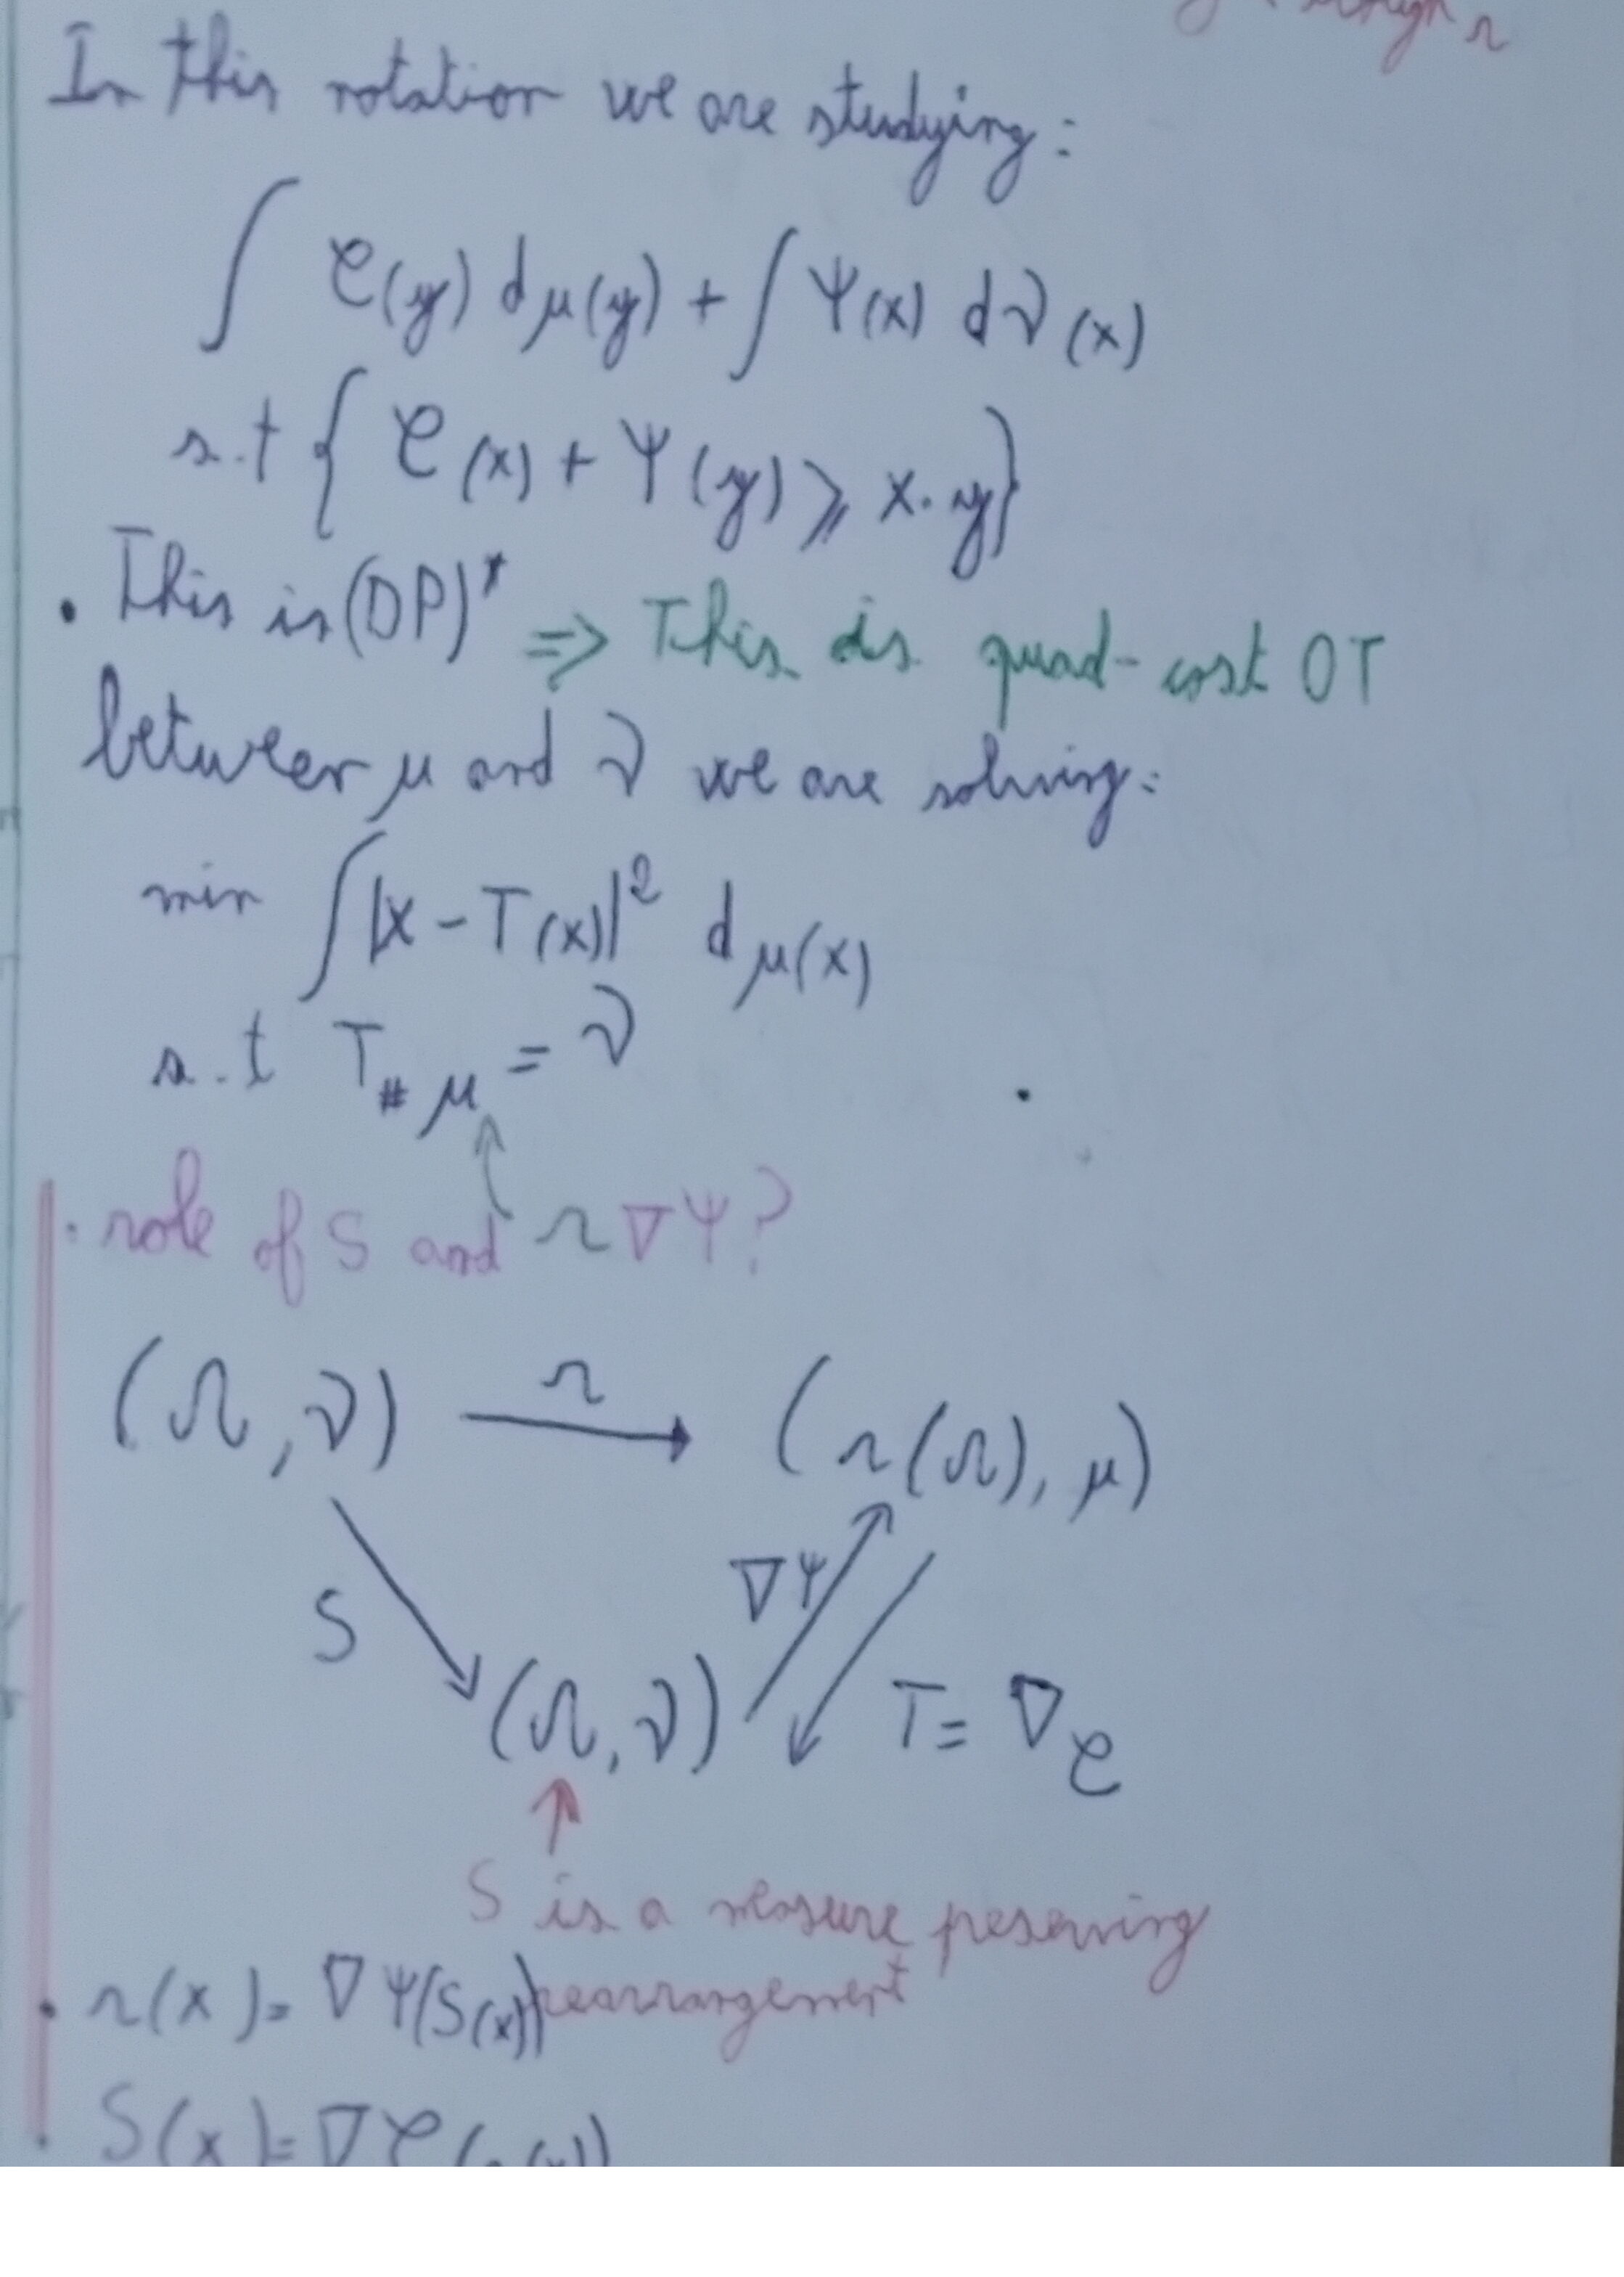
\includegraphics[width=0.4\linewidth]{OT_rearrngement.png}
    \subcaption{Class CNN declaration\cite{PFGPlots}}
    \label{fig:figa}

\caption{Showcasing the dataset checkpoints before building .csv format \cite{PFGPlots}.}
\label{fig:examplefloat}
\end{figure}

6. Computation and Regularization (Sinkhorn)
Since the exact OT problem is often computationally expensive, especially in high dimensions, a common approach is Entropic Regularization. This involves modifying the Kantorovich objective function by adding a scaled Kullback-Leibler (KL) divergence term (entropy) as a regularizer:

$ L_\epsilon^c(\alpha, \beta) := \min_{\pi \in U(\alpha, \beta)} \int_{X \times Y} c(x, y)d\pi(x, y) + \epsilon \text{KL}(\pi | \alpha \otimes \beta) $
This makes the problem strictly convex, guaranteeing a unique, smooth solution $P_\epsilon$. The solution $P_\epsilon$ can be efficiently computed using Sinkhorn's algorithm, which is derived from the dual regularized problem.

Part 2: Concepts to Retain from the Sources
The sources emphasize that Optimal Transport is a crucial concept in contemporary machine learning for introducing geometric knowledge and defining robust metrics, particularly when dealing with structured data like neural network parameters or topological descriptors.
1. The Wasserstein Distance as a Topological Metric

The Wasserstein distance ($W_q$) is a fundamental metric used to compare persistence diagrams (PDs) in Topological Data Analysis (TDA). This distance leverages optimal transport theory to calculate the cost of matching features (points) between two diagrams.

When used in optimization pipelines, the Sliced Wasserstein Distance (SWD) or related kernelized versions are often preferred because the full Wasserstein distance involves combinatorial matching and is generally non-differentiable.

The Optimal Transport distance is used to define distances between discrete signed measures, such as the Hilbert decomposition signed measure derived from multiparameter persistence, enabling the creation of differentiable topological losses.
2. Optimal Transport for Neural Network Structure (OTMANN)

The concept of optimal transport is adapted to create the OTMANN (Optimal Transport Metrics for Architectures of Neural Networks) distance.

OTMANN is formulated as an Optimal Transport program that minimizes a matching scheme to quantify the dissimilarity between two network architectures based on structural position and layer properties.

This metric is used within the NASBOT (Neural Architecture Search with Bayesian Optimisation and Optimal Transport) framework, where a measure of similarity (a kernel) is derived from the OTMANN distance to facilitate Bayesian optimization.

Although OTMANN uses an OT formulation, it is specifically noted that it is not a Wasserstein distance because the underlying mass supports and cost matrices change based on the specific networks being compared.
3. Role in Loss Functions and Continual Learning

Optimal Transport provides a robust way to compare distributions of complex objects. This is highly relevant to my objective, as you noted that the Wasserstein distance (WD) decreases meaningfully during fine-tuning of weight hyper-representations, suggesting it captures functional similarity better than simple $L_2$ losses.

Optimal Transport is seen as a key component for designing loss functions that can preserve both the shape (Topological manifold) and content of data, making it a prime candidate for optimizing knowledge combination in generative models like the one you are developing.

OT finds applications in analyzing generative models via Flow Matching, where an optimal transport map is sought to transform a reference distribution (like Gaussian noise) to a target data distribution.



    \subsection{Persistent Homology Primer}
    
% This section outlines the Persistent Homology (PH) primer and concludes with a recommendation for a suitable loss function mixture for my Transformer model, specifically designed to rival diffusion-based methods like D2NWG.
% My Transformer model, utilizing two encoders for Convolutional Neural Network (CNN) weights (from MNIST sub-partitions) and a dense layer merging embeddings, feeding a decoder for the union CNN, acts as a generative hyper-representation model. This framework seeks to predict functional weights, thus engaging in weight regression and knowledge aggregation for continual learning.
% The generative hyper-representation approach (like D2NWG) leverages latent diffusion to harness knowledge from a collection of pretrained weights, generating dataset- or task-conditioned parameters. Critically, diffusion models for weight generation, such as D2NWG, model the parameter distribution using a VAE encoder/decoder structure and a diffusion process, optimizing the Latent Diffusion Model (LLDM) objective, which is an $L_2$ loss on the noise component $\epsilon$.
% My observed challenge--that Mean Squared Error (MSE) is inadequate and the Wasserstein Distance (WD) decreases meaningfully during fine-tuning--suggests that optimizing solely for reconstruction precision (like $L_{MSE}$ or the $L_2$ inherent in the LLDM objective) is insufficient. This strongly motivates using a topologically-aware loss that enforces manifold structure, aiding in finding weights that lie on the optimal solution surface.
 
\subsubsection{Topological Data Analysis (TDA) Background}

\paragraph{Persistent Homology and Classical TDA}
Topological Data Analysis (TDA) is a field of algebraic topology aimed at providing quantifiable, comparable, robust, and concise summaries of the shape of data. PH is the core tool of TDA, analyzing the evolution of topological features across different scales.
The process begins by representing the data space as a simplicial complex. A filtration is then constructed : a nested sequence of increasing subsets of the simplicial complex.
Homology provides the mathematical language for counting the holes, or cavities, in a topological space. The dimension of the $i$-th homology group, $H_i(K)$, is the $i$-th Betti number ($\beta_i$), which counts the number of independent $i$-dimensional holes (e.g., $\beta_0$ counts connected components, $\beta_1$ counts loops/tunnels).
Persistent Homology tracks how these homology groups evolve (or persist) across the filtration. Features born at one scale and dying at a later scale are considered persistent and are deemed more likely to represent true topological structure rather than noise.

One-Parameter Persistence and Barcodes/Diagrams
In the classical one-parameter setting (indexed by a single scale value, $t \in \mathbb{R}$), there exists a canonical and complete discrete invariant for PH: the persistence barcode.


Barcode: A multiset of intervals $[b, d)$, where $b$ is the filtration value (scale) at which a topological feature is born (appears) and $d$ is the value at which it dies (is filled or disappears).


Persistence Diagram (PD): An equivalent representation where each interval $[b, d)$ is plotted as a point $(b, d)$ in the extended plane. The persistence (lifetime) of the feature is $d-b$, which is the vertical distance from the point to the diagonal $\Delta = {(x, x)}$, where noise typically lies.

\begin{itemize}
\item \textbf(Persistence Diagram)
% A persistence diagram encodes the multiset of birth�death pairs (bi,di)(b_i, d_i)(bi,di) of topological features obtained from a filtration {Kt}t?R\{K_t\}_{t\in\mathbb{R}}{Kt}t?R. Each feature corresponds to a homology class [?]?Hk(Kt)[\sigma] \in H_k(K_t)[?]?Hk(Kt) that appears (�is born�) at t=bit=b_it=bi and vanishes (�dies�) at t=dit=d_it=di. Formally, Dk={(bi,di) ? bi,di?R,bi<di}?R2D_k = \{(b_i, d_i)\ |\ b_i, d_i \in \mathbb{R}, b_i < d_i\} \subset \mathbb{R}^2Dk={(bi,di) ? bi,di?R,bi<di}?R2. The persistence diagram is a stable invariant under the bottleneck and Wasserstein metrics and provides a compact summary of the homological evolution across scales.
 
 
 
 \begin{figure}[H]
    \centering
    \includegraphics[width=0.5\linewidth]{5.4.1 Persistant homology/1_persistance diagram.png}
    \caption{Your caption here (optional)}
    \label{fig:your-label}
\end{figure}



\item \textbf(Barcodes)
% A barcode is an equivalent representation of the persistence diagram that depicts each homological feature as an interval [bi,di)[b_i, d_i)[bi,di) on the real line, where bib_ibi and did_idi denote the filtration values of birth and death, respectively. Given a filtration {Kt}t?R\{K_t\}_{t\in\mathbb{R}}{Kt}t?R and homology functor HkH_kHk, the decomposition theorem for pointwise finite-dimensional persistence modules Vt=Hk(Kt)V_t = H_k(K_t)Vt=Hk(Kt) yields a direct sum of interval modules. Thus, the barcode is a visualization of this decomposition, characterizing persistent kkk-dimensional homology classes and their stability under perturbations of the filtration function.
 
 
  \begin{figure}[H]
    \centering
    \includegraphics[width=0.5\linewidth]{5.4.1 Persistant homology/2_barcode.png}
    \caption{Your caption here (optional)}
    \label{fig:your-label}
\end{figure}

\item \textbf(Persistence Landscape)
% The persistence landscape is a functional representation of a persistence diagram DDD. Each point (bi,di)(b_i, d_i)(bi,di) defines a piecewise-linear tent function fi(t)=max(0,min(t?bi,di?t))f_i(t) = \max(0, \min(t - b_i, d_i - t))fi(t)=max(0,min(t?bi,di?t)). The kkk-th landscape function is ?k(t)=k-maxifi(t)\lambda_k(t) = k\text{-}\'max i f_i(t)?k(t)=k-maxifi(t), giving an ordered sequence of upper envelopes. The collection ?={?k(t)}k?1\Lambda = \{\lambda_k(t)\}_{k\ge1}?={?k(t)}k?1 lies in the Banach space Lp(R�N)L^p(\mathbb{R}\times\mathbb{N})Lp(R�N), enabling linear operations, norms, and statistical analysis while maintaining stability properties relative to the bottleneck distance between diagrams.
 
 
   \begin{figure}[H]
    \centering
    \includegraphics[width=0.5\linewidth]{5.4.1 Persistant homology/3_Landscape.png}
    \caption{Your caption here (optional)}
    \label{fig:your-label}
\end{figure}


\item \textbf(Persistence Image)
% The persistence image embeds persistence diagrams into Euclidean space by convolving each point (bi,di)(b_i, d_i)(bi,di) (often transformed via persistence coordinates pi=(bi,di?bi)p_i = (b_i, d_i - b_i)pi=(bi,di?bi)) with a differentiable weighting kernel ?:R2?R\phi: \mathbb{R}^2 \to \mathbb{R}?:R2?R. The persistence surface is ?(x,y)=?iw(pi)?(x?bi,y?(di?bi))\rho(x, y) = \sum_i w(p_i)\phi(x - b_i, y - (d_i - b_i))?(x,y)=?iw(pi)?(x?bi,y?(di?bi)), and discretization over a fixed grid yields a vectorized image. This stable embedding converts topological information into differentiable, fixed-length features suitable for gradient-based learning and statistical modeling.


\item \textbf(Heat Kernel / Image)
% The heat kernel signature is derived from the Laplace�Beltrami operator ?\Delta? on a manifold or simplicial complex. The heat kernel Kt(x,y)K_t(x,y)Kt(x,y) satisfies the heat equation ?tKt=??Kt\partial_t K_t = -\Delta K_t?tKt=??Kt with initial condition K0=?xyK_0 = \delta_{xy}K0=?xy. For persistence-based heat representations, diagrams are smoothed using Gaussian kernels parameterized by a diffusion scale ttt, yielding differentiable embeddings ?t(x,y)=?ie??(x,y)?(bi,di)?2/4t\rho_t(x,y) = \sum_i e^{-\| (x,y) - (b_i, d_i)\|^2 / 4t}?t(x,y)=?ie??(x,y)?(bi,di)?2/4t. This defines a multiscale, continuous analogue of persistence, providing stability and differentiability via diffusion geometry.

\item \textbf(Betti Numbers / Curves)
% Given a filtration {Kt}t?R\{K_t\}_{t\in\mathbb{R}}{Kt}t?R, the Betti curve ?k(t)=dimHk(Kt)\beta_k(t) = \dim H_k(K_t)?k(t)=dimHk(Kt) tracks the number of independent kkk-dimensional homology classes over scale. The vector of Betti numbers (?0,?1,�?)(\beta_0, \beta_1, \dots)(?0,?1,�) is a topological invariant characterizing connected components, cycles, and voids. The Betti curve is the step function version of the rank invariant ?(b,d)=rank(Hk(Kb?Kd))\rho(b,d) = \text{rank}(H_k(K_b \to K_d))?(b,d)=rank(Hk(Kb?Kd)), encoding topological evolution continuously and providing a simple yet robust topological signature.
 
    \begin{figure}[H]
    \centering
    \includegraphics[width=0.5\linewidth]{5.4.1 Persistant homology/6_Betti.png}
    \caption{Your caption here (optional)}
    \label{fig:your-label}
\end{figure}


\item \textbf(Bottleneck Distance)
% The bottleneck distance dB(D1,D2)d_B(D_1, D_2)dB(D1,D2) between two persistence diagrams D1,D2D_1, D_2D1,D2 is defined as
% dB(D1,D2)=inf?:D1?D2supx?D1?x??(x)??,d_B(D_1, D_2) = \inf_{\gamma: D_1 \to D_2} \sup_{x \in D_1} \|x - \gamma(x)\|_\infty,dB(D1,D2)=?:D1?D2infx?D1sup?x??(x)??, 
% where ?\gamma? ranges over bijections between diagrams extended with the diagonal {(x,x)}\{(x, x)\}{(x,x)}. It metrizes the space of persistence diagrams, ensuring stability of persistent homology under small perturbations of the filtration function. This is the L?L^\inftyL? optimal matching cost between diagrams.

\item \textbf(Wasserstein Distance)
% The ppp-Wasserstein distance between two persistence diagrams D1,D2D_1, D_2D1,D2 is given by
% Wp(D1,D2)=(inf?:D1?D2?x?D1?x??(x)??p)1/p.W_p(D_1, D_2) = \left( \inf_{\gamma: D_1 \to D_2} \sum_{x \in D_1} \|x - \gamma(x)\|_\infty^p \right)^{1/p}.Wp(D1,D2)=(?:D1?D2infx?D1??x??(x)??p)1/p. 
% It generalizes the bottleneck distance (p=?p=\inftyp=?) and induces a topology on the space of diagrams compatible with convergence of persistence. Wasserstein distances allow differentiable relaxations via Sinkhorn or entropic regularization, making them valuable for optimal-transport�based topological learning.

\item \textbf(Sliced Wasserstein Distance)
% The sliced Wasserstein distance projects persistence diagrams onto one-dimensional lines L?={x?????S1}L_\theta = \{x \cdot \theta \mid \theta \in S^1\}L?={x?????S1} and integrates the 1-D Wasserstein distances between projected diagrams:
% SWp(D1,D2)=(?S1Wpp(??(D1),??(D2))?d?)1/p.SW_p(D_1, D_2) = \left( \int_{S^1} W_p^p(\pi_\theta(D_1), \pi_\theta(D_2))\,d\theta \right)^{1/p}.SWp(D1,D2)=(?S1Wpp(??(D1),??(D2))d?)1/p. 
% It approximates WpW_pWp while remaining computationally efficient and differentiable. The sliced formulation preserves topological stability and provides a continuous, smooth cost function suitable for integration into gradient-based optimization pipelines.


\item \textbf(Multiparameter Persistence)
% Multiparameter persistence generalizes classical persistence to filtrations indexed by Rn\mathbb{R}^nRn with the product order x?y ?? ?xi?yi ?ix \preceq y \iff x_i \le y_i \ \forall ix?y?xi?yi ?i. Given a functor V:Rn?VectkV: \mathbb{R}^n \to \text{Vect}_\BbbkV:Rn?Vectk, its rank invariant is ?V(a,b)=rank(V(a?b))\rho_V(a,b) = \text{rank}(V(a \preceq b))?V(a,b)=rank(V(a?b)). Unlike the one-parameter case, no complete discrete invariant (like barcodes) exists; instead, one studies algebraic invariants such as Betti tables or Hilbert series derived from the finitely generated graded module MVM_VMV over the polynomial ring k[x1,�,xn]\Bbbk[x_1,\ldots,x_n]k[x1,�,xn]. Multiparameter persistence thus encodes topological variability across multiple simultaneous scales.
 
 
    \begin{figure}[H]
    \centering
    \includegraphics[width=0.5\linewidth]{5.4.1 Persistant homology/10_multipers_1.png}
    \caption{Your caption here (optional)}
    \label{fig:your-label}
\end{figure}

   \begin{figure}[H]
    \centering
    \includegraphics[width=0.5\linewidth]{5.4.1 Persistant homology/10_multipers_2.png}
    \caption{Your caption here (optional)}
    \label{fig:your-label}
\end{figure}

   \begin{figure}[H]
    \centering
    \includegraphics[width=0.5\linewidth]{5.4.1 Persistant homology/10_multipers_3.png}
    \caption{Your caption here (optional)}
    \label{fig:your-label}
\end{figure}

   \begin{figure}[H]
    \centering
    \includegraphics[width=0.5\linewidth]{5.4.1 Persistant homology/10_multipers_4.png}
    \caption{Your caption here (optional)}
    \label{fig:your-label}
\end{figure}


\item \textbf(Mapper Algorithm / Graph)
% Mapper constructs a simplicial graph summarizing a dataset X?RdX \subset \mathbb{R}^dX?Rd given a filter function f:X?Rmf: X \to \mathbb{R}^mf:X?Rm. A cover {Ui}\{U_i\}{Ui} of f(X)f(X)f(X) induces preimages f?1(Ui)f^{-1}(U_i)f?1(Ui), each clustered (e.g., by connected components), yielding nodes representing clusters and edges between overlapping clusters. The Mapper graph approximates the Reeb graph of fff, providing a combinatorial topological summary. Formally, the nerve N({Ci})N(\{C_i\})N({Ci}) of the cover captures the global topological structure induced by the filter and clustering scale, bridging discrete topology and data geometry.
 
    \begin{figure}[H]
    \centering
    \includegraphics[width=0.5\linewidth]{5.4.1 Persistant homology/11_mapper.png}
    \caption{Your caption here (optional)}
    \label{fig:your-label}
\end{figure}

\item \textbf(Reeb Graph)
% For a continuous scalar function f:X?Rf: X \to \mathbb{R}f:X?R on a manifold or simplicial complex, the Reeb graph RfR_fRf is the quotient space obtained by collapsing each connected component of level sets f?1(c)f^{-1}(c)f?1(c) to a point. The quotient map ?:X?Rf\pi: X \to R_f?:X?Rf satisfies f=f~??f = \tilde{f} \circ \pif=f~??, preserving the function�s critical structure. Reeb graphs encode the evolution and merging of level-set components across function values, providing a 1D topological skeleton. They are stable under small perturbations of fff in the functional distortion metric.
 
 
    \begin{figure}[H]
    \centering
    \includegraphics[width=0.5\linewidth]{5.4.1 Persistant homology/12_reeb_graph.png}
    \caption{Your caption here (optional)}
    \label{fig:your-label}
\end{figure}


\item \textbf(Contour Trees)
% A contour tree is a simplified form of the Reeb graph for simply connected domains. For a scalar field f:X?Rf: X \to \mathbb{R}f:X?R on a contractible manifold, the contour tree tracks how connected components of level sets merge or split as fff varies. Formally, it�s a tree whose nodes correspond to critical points of fff and edges correspond to monotone regions between them. Contour trees provide efficient topological summarization of scalar fields, often used for visualization and feature extraction in volumetric or manifold-valued data.
 
    \begin{figure}[H]
    \centering
    \includegraphics[width=0.5\linewidth]{5.4.1 Persistant homology/13_Contour_trees.png}
    \caption{Your caption here (optional)}
    \label{fig:your-label}
\end{figure}

\item \textbf(Merge Trees)
% The merge tree of f:X?Rf: X \to \mathbb{R}f:X?R tracks the evolution of the sublevel sets Xa=f?1((??,a])X_a = f^{-1}((-\infty, a])Xa=f?1((??,a]). Each node corresponds to a critical point, and branches merge at saddle points where connected components of XaX_aXa coalesce. Algebraically, it captures the 000-dimensional persistence of fff, encoding connectivity changes through filtration. Merge trees form a hierarchical structure suitable for topological simplification and statistical comparison via tree edit or interleaving distances.

   \begin{figure}[H]
    \centering
    \includegraphics[width=0.5\linewidth]{5.4.1 Persistant homology/14_merge_trees.png}
    \caption{Your caption here (optional)}
    \label{fig:your-label}
\end{figure}


\item \textbf(Morse--Smale Complex)
% Given a smooth manifold MMM and a Morse function f:M?Rf: M \to \mathbb{R}f:M?R, the Morse�Smale complex partitions MMM into cells defined by the intersections of ascending and descending manifolds of the gradient flow ?f\nabla f?f. These cells correspond to the gradient paths between critical points. Formally, it yields a cell decomposition reflecting the topology and geometry of MMM and is used for hierarchical simplification, feature extraction, and structural comparison of scalar fields.

\item \textbf(Topological Regularizer)
% A topological regularizer introduces a differentiable penalty on topological complexity within machine learning models. Given an output function f?f_\thetaf?, one computes its persistent homology Dk(f?)D_k(f_\theta)Dk(f?) and defines a loss term Ltopo(?)=?i?(di?bi)L_\text{topo}(\theta) = \sum_i \phi(d_i - b_i)Ltopo(?)=?i?(di?bi) penalizing undesired birth�death intervals. Differentiable approximations (e.g., via persistence landscapes or soft Wasserstein distances) enable gradient-based optimization to enforce specific topological constraints--such as enforcing connectivity, loop removal, or manifold smoothness--during training.
 
\item \textbf(Local Cohomology)
% Local cohomology measures the topology of a space XXX near a subset Z?XZ \subset XZ?X. Given a sheaf F\mathcal{F}F on XXX, local cohomology groups are HZi(X;F)=lim?U?ZHi(X,X?U;F)H_Z^i(X; \mathcal{F}) = \varinjlim_{U \supset Z} H^i(X, X\setminus U; \mathcal{F})HZi(X;F)=limU?ZHi(X,X?U;F). In data analysis, these capture local topological behavior such as singularities or boundaries. Computable via simplicial approximations, local cohomology provides a dual perspective to persistent homology, emphasizing obstructions and local invariants rather than global connectedness.
 

\item \textbf(Vietoris--Rips Complex)
% Given a point cloud X?RdX \subset \mathbb{R}^dX?Rd and scale ?>0\epsilon > 0?>0, the Vietoris�Rips complex VR?(X)VR_\epsilon(X)VR?(X) is the abstract simplicial complex whose simplices correspond to finite subsets of XXX of diameter ? 2?2\epsilon2?. Explicitly,
% VR?(X)={??X??x?y??2?, ?x,y??}.VR_\epsilon(X) = \{ \sigma \subset X \mid \|x - y\| \le 2\epsilon, \ \forall x,y \in \sigma \}.VR?(X)={??X??x?y??2?, ?x,y??}. 
% As ?\epsilon? increases, one obtains a filtration whose homology captures the shape of the underlying manifold. Vietoris�Rips complexes are foundational in computational topology due to their metric simplicity and stability.
 
\item \textbf(Alpha Complex)
% An alpha complex is a subcomplex of the Delaunay triangulation of X?RdX \subset \mathbb{R}^dX?Rd parameterized by a scale ?\alpha?. A simplex ?\sigma? belongs to the alpha complex if its circumscribed ball has radius ? ?\alpha? and its center lies within the corresponding Voronoi region intersection. The alpha filtration captures the same homotopy type as the union of balls of radius ?\alpha? centered at XXX, yielding a computationally efficient approximation of the ?ech complex and enabling geometrically faithful persistent homology.

\item \textbf (Cubical Complex)
% A cubical complex is a topological space formed by gluing elementary cubes [a1,a1+1]�?�[an,an+1][a_1, a_1+1] \times \dots \times [a_n, a_n+1][a1,a1+1]�?�[an,an+1] along faces. For image or voxel data I:Zn?RI: \mathbb{Z}^n \to \mathbb{R}I:Zn?R, one defines sublevel sets Xt={x?I(x)?t}X_t = \{x \mid I(x) \le t\}Xt={x?I(x)?t}, which induce a cubical filtration. Homology on cubical complexes is efficiently computable via discrete boundary operators and is particularly well-suited for TDA on gridded or digital data, preserving adjacency and topological consistency of pixel/voxel structures.
% Stability of Persistent Homology
% A key motivation for using TDA in machine learning is the stability property of persistent homology.
% The stability proofs (often involving the bottleneck distance) show that small changes in the input data lead to only small changes in the resulting persistence diagram. Specifically, given two tame functions $f$ and $g$ defining filtrations on a space $M$, the bottleneck distance ($W_\infty$) between their corresponding persistence diagrams is bounded by the $L_\infty$-distance between the functions: $d_{b}(Dgm(f), Dgm(g)) \leq |f-g|_{\infty}$. This result ensures robustness against perturbations and noise.
\end{itemize}


    \begin{figure}[H]
    \centering
    \includegraphics[width=0.5\linewidth]{5.4.1 Persistant homology/PH_summary.png}
    \caption{Your caption here (optional)}
    \label{fig:your-label}
\end{figure}


3. The Mapper Algorithm


\begin{algorithm}
\caption{Mapper algorithm}
\KwIn{D with $|D| = m$, filter function $f: D \to \mathbb{R}^d$, finite cover $\mathcal{U} = \{U_i\}_{i \in I}$ of $\text{Im}(f) \subseteq \mathbb{R}^d$, clustering algorithm $\mathcal{C}$.}
\KwOut{Simplicial complex $S_D$.}
$S_D \leftarrow \emptyset$\;
$D_i \leftarrow f^{-1}(U_i)$ for all $i \in I$\;
\For{all $i \in I$}{
    $\{C_i^1, \ldots, C_i^{k_i}\} \leftarrow \mathcal{C}(D_i)$ \tcp{Apply the clustering algorithm to $D_i$: the output are the clusters}
    $S_D \leftarrow S_D \cup \{C_i^1, \ldots, C_i^{k_i}\}$ \tcp{Add the clusters found as vertices}
}
\For{all $\{C_1, \ldots, C_t\} \in \mathcal{P} \setminus S \bigcup_{i \in I} \{C_i^1, \ldots, C_i^{k_i}\}$ \tcp*[f]{for all possible subsets of found clusters}}{
    \If{$\bigcap_{j=1}^t C_j \neq \emptyset$}{
        $S_D \leftarrow S_D \cup \{\{C_1, \ldots, C_t\}\}$ \tcp{We add the simplex $\{C_1, \ldots, C_t\}$}
    }
}
\Return{$S_D$}\;
\end{algorithm}


The Mapper algorithm (introduced by Singh et al., 2007) is a tool for visualizing and extracting structural descriptions from high-dimensional datasets, typically outputting a graph or simplicial complex.
Mapper uses four primary ingredients:
1.	A dataset $D$.
2.	A filter function ($f$): A scalar (usually $\mathbb{R}$ or $\mathbb{R}^2$-valued) function defined on the dataset $D$ that projects the high-dimensional data down to a manageable domain.
3.	A finite, overlapping cover of the image of the filter function $f$.
4.	A clustering algorithm (like DBSCAN) applied to the preimages of the cover elements.
The result is a graph where nodes represent clusters of points that are close in the data space and map close to each other via the filter function, and edges connect nodes if their corresponding clusters overlap. Mapper is highly valuable for exploratory data analysis and visualization, offering interpretability, but the complex construction typically renders the graph structure non-differentiable for end-to-end optimization.
4. Transition to Multidimensional Persistence
In many applications, data is complex and may be filtered along multiple non-linear dimensions simultaneously (e.g., scale and density), leading to a multifiltration.
The critical transition occurs when $n > 1$ parameters index the filtration (e.g., a bifiltration parameterized by radius $\epsilon$ and curvature $\kappa$). Gunnar Carlsson and Afra Zomorodian demonstrated that, unlike the one-parameter case, no similar complete discrete invariant (like the barcode) exists for multiparameter persistence modules due to fundamental algebraic reasons.
Instead, they proposed the rank invariant ($\rho_{X,i}$) as a robust discrete invariant for multifiltrations.


Rank Invariant: Defined as $\rho_{X,i}(u, v) = \text{rank}(H_i(X_u, k) \to H_i(X_v, k))$, this invariant measures the rank of the structure maps between homology groups indexed by parameters $u \leq v$.


While the rank invariant is mathematically equivalent to the persistence barcode in one dimension (where it is complete), it extends to higher dimensions as a useful, though incomplete, invariant for robust estimation of Betti numbers and detection of persistent features.
To address the lack of a canonical discrete descriptor, modern research focuses on developing effective and often differentiable incomplete descriptors for multiparameter persistence, such as the multiparameter persistence landscape, multiparameter persistence image, and signed barcodes as measures.

Recommended Loss Function and Topological Descriptors
To rival diffusion-based methods like D2NWG, which prioritize reconstruction accuracy(often $L_2$ based), my Transformer model must optimize for qualities conducive to fine-tuning and fast learning--qualities often missed by simple MSE on weights.
Choosing the Optimal Loss Function
Since my Transformer uses an autoencoder structure for weight regression, the loss should leverage known functional losses for hyper-representations combined with topologically robust metrics:


1.	Layer--Wise Loss Normalization (LWLN): You should adopt the LWLN MSE loss. This loss prevents layers with small weight magnitudes from being disregarded, which is critical for generating functional models (as shown in work related to hyper--representations).  $L_{\overline{MSE}} = \frac{1}{MN} \sum_{i=1}^M \sum_{l=1}^L \frac{|\hat{w}^{(l)}_i - w^{(l)}_i|_2^2}{\sigma^2_l} \quad $


2.	Contrastive Loss ($L_c$): The original hyper-representation work combines $L_{\overline{MSE}}$ with a contrastive loss $L_c$ to impose structure and regularity on the latent space. This practice should be retained: $L = \beta L_{\overline{MSE}} + (1-\beta)L_c$.


3.	Topological Regularizer (Differentiable WD): To enforce manifold properties and bridge the gap to high--performing weights efficiently, incorporating the topological distance that showed success in my  convergence experiments :the Wasserstein Distance (WD) is essential. The WD metric on persistence diagrams is the large--scale version of optimal transport distance. Since full WD is often non--differentiable, you should employ the Sliced Wasserstein Distance (SWD), which is known to be differentiable. $ L_{Topological} = \alpha \cdot \text{SWD}(\text{PH}(\hat{W}), \text{PH}(W_{target}))$  Where $\hat{W}$ are the predicted weights and $W_{target}$ are the ground truth/optimal weights.


4.	Weight Importance Regularization (Fisher Information): Given my work's focus on continual learning and efficient representations, a term promoting finetunable weights is necessary. The Fisher Information Matrix (F) provides information about weight importance. Adopting an Elastic Weight Consolidation (EWC) style regularization term, where parameters are penalized based on their importance (F) to previous tasks, aligns perfectly with penalizing deviation from desired weight structures.  $R = \sum_i \frac{\gamma}{2} F_i (\hat{w}_i - w^{}_i)^2$  Where $w^{}_i$ are the important weights/embeddings from the encoder stage (sub--partitions) and $F_i$ is the corresponding diagonal Fisher information value.
Recommended Composite Loss: A mixture that targets both precise reconstruction and topological/functional relevance:  $L_{Total} = \beta L_{\overline{MSE}} + (1-\beta)L_c + \alpha L_{Topological} + R $


Summary of Differentiable Topological Descriptors :


The complexity of TDA features often requires turning the persistence diagram (PD) into a vectorization or using specific differentiable measures to integrate into gradient-based learning pipelines. The following table summarizes key descriptors and their suitability for Transformer training (where differentiability is crucial):
Table 1: Topological Descriptors and Suitability for Transformer Training

\renewcommand\theadfont{\bfseries}
\newcolumntype{L}[1]{>{\RaggedRight\arraybackslash}p{#1}}

\begin{table}[htbp]
\centering
\caption{Topological Descriptors and Suitability for Transformer Training}
\label{tab:tda-features}

% 4 columns ? total width = \linewidth
\setlength{\tabcolsep}{5pt}
\begin{tabular}{|
    *{4}{L{\dimexpr\linewidth/4 - 2\tabcolsep\relax}|}
}
\hline
\thead{TDA Feature} & \thead{Description} & \thead{Differentiable?} & \thead{Notes/Context} \\
\hline

Persistence Diagram/Barcode &
  Multiset of birth/death points. &
  Partial. Computation involves non-smooth operations. Requires implicit differentiation libraries (e.g., Torchph). &
  Core descriptor, often used as input for differentiable vectorizations. \\
\hline

Persistence Landscape &
  Continuous, piecewise linear function summarizing PD features. &
  Yes. Allows for averaging and is useful for statistical analysis. &
  One of the most computationally tractable differentiable descriptors. \\
\hline

Persistence Image (Heat Kernel) &
  Grid-based vectorization of PD using Gaussian kernels. &
  Yes. Provides a smooth, fixed-size vector output highly valued in ML. &
  Implemented for differentiability in libraries like Perslay and giotto-tda. \\
\hline

(Sliced) Wasserstein Distance &
  Metric based on optimal transport between PDs. &
  Yes (Sliced and kernelized versions). Full bottleneck distance is generally non-differentiable. &
  Crucial for manifold learning and metric preservation. \\
\hline

Signed Barcodes/Hilbert Decomposition &
  Discrete signed measure characterizing the Hilbert function of a filtration. &
  Yes (as measures). &
  These multiparameter descriptors are shown to be semilinearly determined on grids, allowing for explicit Clarke subdifferentiability. \\
\hline

Multiparameter Persistence &
  Persistence indexed by $n>1$ parameters (e.g., density + scale). &
  Yes (via specific descriptors/libraries like multipers). &
  Generally challenging, but differentiable invariants are emerging. \\
\hline

Topological Regularizer &
  Topological distance used as a loss function component. &
  Yes. &
  Directly designed for integration into gradient descent pipelines. \\
\hline

\end{tabular}
\end{table}


Comparison of Simplicial Complexes
The choice of simplicial complex construction determines the fidelity of the topological approximation and computational cost. For geometric data (like weights visualized as point clouds), Vietoris--Rips and related complexes are common.
Table 2: Comparison of TDA Simplicial Complexes

\renewcommand\theadfont{\bfseries}
\newcolumntype{L}[1]{>{\RaggedRight\arraybackslash}p{#1}}

\begin{table}[htbp]
\centering
\caption{Topological Descriptors and Suitability for Transformer Training}
\label{tab:tda-features}

% 4 columns ? total width = \linewidth
\setlength{\tabcolsep}{5pt}
\begin{tabular}{|
    *{5}{L{\dimexpr\linewidth/5 - 2\tabcolsep\relax}|}
}
\hline
				
\thead{Complex Type} & \thead{Input Data} & \thead{Key Construction Rule} & \thead{Advantages} & \thead{Disadvantages} \\
\hline
Vietoris--Rips (RIPS)&
Point cloud + distance matrix in any metric space.&
Clique complex: A $k$-simplex for every subset of $k+1$ points where all pairwise distances are $\leq$ radius $r$.	&
Easy to define; widely applicable; fast implementations exist (e.g., Ripser).&
Computationally expensive; number of simplices grows combinatorially/exponentially with points.
\\
\hline

Alpha Complex	&
Point cloud in $\mathbb{R}^d$.	&
Subcomplex of the Delaunay triangulation restricted by a radius $\alpha$.&
Captures the true homotopy type of the union of balls; sparse; uses exact geometry.	&
Requires full Delaunay tessellation (even in 3D); restricted to Euclidean space. \\
\hline
?ech Complex &
Point cloud in $\mathbb{R}^d$.&
A $k$-simplex if the intersection of $k+1$ balls of radius $r$ is non-empty.&
Theoretically sound (Nerve Lemma); captures the true homotopy type of the union of balls.&	Computationally expensive; difficult to materialize high-dimensional nerve structures. \\
\hline
Witness Complex &
A large point cloud and a set of Landmarks $L$.	&
Approximates the Rips filtration by only considering proximity to landmarks.&
Ultra-fast; scalable and memory efficient for billion-point clouds.	&
Coarse topological features; sensitive to the selection of landmarks. \\
\hline
Cubical Complex &
Regular grid/voxel data (e.g., images).	 &
Cells are hypercubes (pixels, voxels) based on scalar values.&
Extremely efficient for structured data; ideal for medical imaging/CNN analysis on grids.&
Only for structured grid data.\\
\hline

\end{tabular}
\end{table}

Recent Works in TDA for Neural Network Analysis
The field of TDA for Neural Networks focuses on four broad domains: 1. Architecture, 2. Input/Output Spaces, 3. Internal Representations (Weights/Activations), and 4. Training Dynamics/Loss Functions. My project primarily relates to domains 3 and 4

The following table, similar to the survey provided, summarizes relevant recent contributions:
Table 3: Summaries of Recent Works and Contributions


\renewcommand\theadalign{l}
\newcolumntype{L}[1]{>{\RaggedRight\arraybackslash}p{#1}}

\begin{longtable}{
  |L{0.35\linewidth}|L{0.35\linewidth}|L{0.15\linewidth}|L{0.10\linewidth}|
}
\hline
\thead{Title (Reference)} & \thead{Summary / Contribution} & \thead{Key Area / Cat.} & \thead{Apps.} \\
\hline
\endhead
\hline
\endfoot
\hline
\endlastfoot

DIFFUSION-BASED NEURAL NETWORK WEIGHTS GENERATION (D2NWG) &
Introduces a latent diffusion model leveraging knowledge from pretrained weights to efficiently generate task-conditioned, high-performing weights for transfer learning/initialization. &
Generative Hyper-Rep. & - \\
\hline

Differentiability and Optimization of Multiparameter Persistent Homology &
Developed a general theoretical framework proving that multiparameter persistence descriptors (like signed barcodes and persistence landscapes) are differentiable (semilinearly determined on grids), enabling their use in gradient descent pipelines. &
TDA Theory / Optimization & - \\
\hline

Stable Vectorization of Multiparameter Persistent Homology using Signed Barcodes as Measures &
Introduced the Hilbert decomposition signed measure ($\mu_{Hil}$) and rank decomposition signed measure as differentiable vectorizations of multiparameter persistence modules, offering stability guarantees. &
Multiparameter TDA & - \\
\hline

Intrinsic dimension, persistent homology and generalization in neural networks &
Showed that the persistent homology dimension (a geometric fractal dimension derived from PDs) of the space of training weights correlates significantly with the generalization capacity of NNs (lower dimension = better generalization). &
Training Dynamics (4) & - \\
\hline

A topological regularizer for regularizers via persistent homology (Chen et al., 2019) &
Proposed one of the first topological regularization terms for classifiers, using differentiable PH to remove weak connected components from the decision boundary, reducing overfitting. Regularization of neural networks by modifying their decision regions using differentiable persistent homology. &
Loss Functions (4), (2) & (1) \\
\hline

Neural persistence: A complexity measure for deep neural networks using algebraic topology (Rieck et al., 2019) &
Defined Neural Persistence as a measure of topological complexity derived from the weights of FCFNNs, finding that higher persistence correlates with better generalization, usable as an early stopping criterion. Topological complexity measure for neural networks based on their weights. &
Internal Rep. (3) & (1) \\
\hline

Representation topology divergence: A method for comparing neural network representations &
Proposed RTD, a measure to compare two Vietoris--Rips filtrations (representations) by counting how features merge, providing a dissimilarity measure between data representations. &
Internal Rep. (3) & - \\
\hline

Topological dynamics of functional neural network graphs during reinforcement learning &
Studied the evolution of Betti numbers derived from complexes induced by functional neural network graphs during RL training/inference. &
Internal Rep. (3) & - \\
\hline

% === SECOND BATCH (from continuation) ===
On the complexity of neural network classifiers: A comparison between shallow and deep architectures (Bianchini and Scarselli, 2014) &
Bounds on the Betti numbers of the positive decision region generated by binary classification neural networks with Pfaffian activations. &
(2) & - \\
\hline

Topological approaches to deep learning (Carlsson and Bru?el Gabrielsson, 2020) &
Topological analysis of the weights of convolutional neural networks and generalization of convolutional neural networks. &
(3) & - \\
\hline

Topological data analysis of decision boundaries with application to model selection (Ramamurthy et al., 2019) &
Study and approximation of the topology of network decision boundaries. &
(2) & (5) \\
\hline

Geometry Score: A method for comparing generative adversarial networks (Khrulkov and Oseledets, 2018) &
Measurement of GAN quality using persistent homology. &
(2) & (7) \\
\hline

What does it mean to learn in deep networks? And, how does one detect adversarial attacks? (Corneanu et al., 2019) &
Study of generalization in terms of the persistent homology of neuron activations and their correlations. &
(3) & (1, 3) \\
\hline

On connected sublevel sets in deep learning (Nguyen, 2019) &
Study of the connectivity, boundedness, and local minima of sublevel sets of convex losses for overparameterised neural networks with piecewise linear activation functions. &
(4) & - \\
\hline

Characterizing the shape of activation space in deep neural networks (Gebhart et al., 2019) &
Topological characterization of the neuron activations given a sample. &
(3) & (3) \\
\hline

Exposition and interpretation of the topology of neural networks (Bru?el Gabrielsson and Carlsson, 2019) &
Topological analysis of the weights of convolutional neural networks and connection to generalization capacity of models. &
(3) & - \\
\hline

Path homologies of deep feedforward networks (Chowdhury et al., 2019) &
Analysis of path and directed flag homology groups of MLPs' directed graph. &
(1) & - \\
\hline

Topology of deep neural networks (Naitzat et al., 2020) &
Study of the topology of the data through layer transformations. &
(3) & - \\
\hline

Finding the homology of decision boundaries with active learning (Li et al., 2020) &
Use of active learning to improve the methods of Topological data analysis of decision boundaries with application to model selection. &
(2) & (5) \\
\hline

Computing the testing error without a testing set (Corneanu et al., 2020) &
Regression of test accuracy using topological vectorizations of persistence diagrams. &
(3) & (6) \\
\hline

Topological detection of trojaned neural networks (Zheng et al., 2021) &
Study of trojaned networks in terms of the persistent homology of neuron activations and their correlations. &
(3) & (4) \\
\hline

Experimental stability analysis of neural networks in classification problems with confidence sets for persistence diagrams (Akai et al., 2021) &
Study of persistence diagrams of last hidden layer activations and its connection with generalization. &
(3) & - \\
\hline

PHom-GeM: Persistent homology for generative models (Charlier et al., 2019) &
Comparison between persistence diagrams of real and generated manifolds using generative models. &
(2) & (7) \\
\hline

TopoAct: Visually exploring the shape of activations in deep learning (Rathore et al., 2021) &
Analysis of the Mapper graph of neuron activations for each layer. &
(3) & - \\
\hline

Deep neural network pruning using persistent homology (Watanabe and Yamana, 2020) &
Pruning of neural networks using persistent homology. &
(3) & (2) \\


% === NEW ENTRIES (2021�2024) ===
Intrinsic dimension, persistent homology and generalization in neural networks (Birdal et al., 2021) &
Generalization error bounds using persistent homology dimension on the training weights. &
(3, 4) &
(1) \\
\hline

Activation landscapes as a topological summary of neural network performance (Wheeler et al., 2021) &
Study of the topology of the data through layer transformations and its connection with training accuracy. &
(3) &
- \\
\hline

Topology of learning in feedforward neural networks (Gabella, 2021) &
Analysis of the evolution of the weights of a neural network during training using Mapper. &
(3) &
- \\
\hline

Topological uncertainty: Monitoring trained neural networks through persistence of activation graphs (Lacombe et al., 2021) &
Uncertainty measurement of neural network predictions using the topology of neuron activations. &
(3) &
(3, 5) \\
\hline

Topological measurement of deep neural networks using persistent homology (Watanabe and Yamana, 2022b) &
Computation of persistence diagrams using neuron path relevance and connection with network expressivity and problem difficulty. &
(3) &
- \\
\hline

Evaluating the disentanglement of deep generative models with manifold topology (Zhou et al., 2021) &
Measurement of disentanglement of generative neural networks. &
(2) &
- \\
\hline

Quantitative performance assessment of CNN units via topological entropy calculation (Zhao and Zhang, 2022) &
Measurement of quality of convolutions in a neural network using persistent homology. &
(3) &
- \\
\hline

Overfitting measurement of deep neural networks using no data (Watanabe and Yamana, 2022a) &
Study of overfitting by analysing the points near the diagonal of a persistence diagram generated from the weights of a neural network. &
(3) &
- \\
\hline

An adversarial robustness perspective on the topology of neural networks (Goibert et al., 2022) &
Analysis of adversarial examples by means of the topology of the subgraph of under-optimized edges of neural networks. &
(3) &
(3) \\
\hline

Representation topology divergence: A method for comparing neural network representations (Barannikov et al., 2022) &
Definition of similarity between data representations using persistent homology. &
(3) &
(7) \\
\hline

On the topological expressive power of neural networks (Petri and Leitao, 2020) &
Measurement of expressivity of network architectures. &
(2) &
- \\
\hline

Generalization bounds using data-dependent fractal dimensions (Dupuis et al., 2023) &
Data-dependent generalization error bounds using persistent homology dimension on the training weights. &
(3, 4) &
- \\
\hline

TopoBERT: Exploring the topology of fine-tuned word representations (Rathore et al., 2023) &
Mapper graph of transformer-based models with applications in finetuning of language models. &
(3) &
- \\
\hline

Experimental observations of the topology of convolutional neural network activations (Purvine et al., 2023) &
Analysis of the Mapper graph of neuron activations and definition of a similarity function between layers using sliced Wasserstein distances between persistence diagrams generated from them. &
(3) &
- \\
\hline

ReLU neural networks, polyhedral decompositions, and persistent homology (Liu et al., 2023b) &
Detection of homological features in manifolds embedded in the input space of a neural network using the polyhedra decomposition induced by a ReLU feedforward neural network. &
(2) &
- \\
\hline

Caveats of neural persistence in deep neural networks (Girrbach et al., 2023) &
Connection between neural persistence and variance measures of neural network weights. &
(3) &
- \\
\hline

On the use of persistent homology to control the generalization capacity of a neural network (Barbara et al., 2024) &
Regression of generalization gap using the average persistence of zero dimensional persistence diagrams. &
(3) &
(6) \\
\hline

Visualizing and analyzing the topology of neuron activations in deep adversarial training (Zhou et al., 2023) &
Analysis of the Mapper graph of neuron activations of normally and adversarially trained neural networks. &
(3) &
- \\
\hline

TopP\&R: Robust Support Estimation Approach for Evaluating Fidelity and Diversity in Generative Models (Kim et al., 2023) &
Approximation of the precision and recall scores for generative models using a persistent homology-based approach. &
(2) &
(7) \\
\hline

Topological structure of complex predictions (Liu et al., 2023a) &
Analysis of the GTDA Reeb network of output spaces of neural networks. &
(2) &
- \\
\hline

Topological dynamics of functional neural network graphs during reinforcement learning (Muller et al., 2024) &
Study of reinforcement learning neural networks during training and inference using homology. &
(3) &
- \\
\hline
Topological dynamics of functional neural network graphs during reinforcement learning (Muller et al., 2024) &
Study of reinforcement learning neural networks during training and inference using homology. &
(3) &
- \\
\hline
Fast Witness Persistence for MRI Volumes via Hybrid Landmarking (Jorge Ruiz Williams 2025) & 
The paper introduces a scalable GPU-accelerated method for computing persistent homology on full-brain MRI volumes using hybrid density-aware landmark selection and witness complexes, achieving runtime under 10 seconds while preserving topological features that traditional methods would take hours to compute.& - & - \\

A Framework for Fast and Stable Representations of Multiparameter Persistent Homology Decompositions (David Loiseaux et al 2023 )  & - & - & -   \\
\hline

Multi-parameter Module Approximation: an efficient and interpretable invariant for multi-parameter persistence modules with guarantees (David Loiseaux et al 2024)  & - & - & - \\
\hline

Stable Vectorization of Multiparameter Persistent Homology using Signed Barcodes as Measures
(David Loiseaux et al 2023)  & - & - & - \\
\hline

Differentiability and Optimization of Multiparameter Persistent Homology
(Luis Scoccola et al 2024)  & - & - & - \\
\hline


\hline
\hline

\end{longtable}

\newpage

Table 1: Table containing the published articles reviewed in this survey ordered by year of publi- cation. Each row corresponds to an article. The first column contains the title; the second column contains a one-line summary; the third column contains the categories introduced in Section 1 as- sociated to each article; and the last column contains the applications introduced in Section 2.4. The four possible categories are 1. Structure of the neural network; 2. Input and output spaces;
3. Internal representations and activations; 4. Training dynamics and loss functions. The seven possible applications are 1. Regularization; 2. Pruning of neural networks; 3. Detection of adversar- ial, out-of-distribution and shifted examples; 4. Detection of trojaned networks; 5. Model selection;
6. Prediction of accuracy; 7. Quality assessment of generative models.


The Mapper algorithm

The breakthrough in utilizing two-dimensional (2D), or more generally multiparameter, persistent homology (PH) stems fundamentally from overcoming a major theoretical limitation of classical one-parameter PH, and subsequently developing differentiable descriptors that allow these rich invariants to be integrated into machine learning optimization tasks
.

1. The Core Limitation of 1D Persistence
In classical persistent homology (often called one-parameter persistence), data is filtered along a single dimension, such as increasing radius (?) or density (?)
. 

This results in a sequence of nested spaces, known as a filtration.
The key theoretical breakthrough for 1D persistence was the establishment of a complete discrete invariant, known as the persistence barcode (or persistence diagram)
. 

This barcode uniquely and completely encodes all the topological information within the filtration, up to isomorphism.
However, many real-world structures are defined by multiple interacting parameters, leading to a multifiltration (e.g., parameterized along curvature ? and radius ?, or scale and density)
. 


If one attempts to use 1D PH on such a structure, one must fix the value of the other parameters, which risks losing valuable information or requiring arbitrary parameter choices.
2. The Negative Result (The Theoretical Wall)
The first step toward the 2D PH breakthrough was the critical realization by Gunnar Carlsson and Afra Zomorodian (2009) that the simplicity and completeness of the 1D barcode do not generalize to higher dimensions.


No Complete Discrete Invariant: Due to fundamental algebraic reasons, no similar canonical complete discrete invariant (like the barcode) exists for n--valued filtering functions when n>1 (e.g., for 2D persistence). The classification of multigraded modules (the algebraic structure corresponding to multifiltrations) involves both discrete and continuous portions, and the continuous portion has no precise, field-independent parameterization.


Field Dependence: The classification in higher dimensions can be dependent on the choice of the coefficient field (k), meaning changing the field changes the classification and the target of the classification, preventing the existence of a complete discrete invariant.
This negative result meant that new mathematical tools were needed to capture persistent topological features in n--parameter settings.
3. The Shift to Incomplete, but Useful, Invariants
Given the impossibility of a complete discrete invariant, the breakthrough shifted focus to developing invariants that are computable, compact, and effective for extracting persistent features--even if they are incomplete.
The proposed alternatives measure the relationships (homomorphisms) between the filtered spaces, rather than just the birth/death times.

The Rank Invariant:

Carlsson and Zomorodian proposed the rank invariant (?X,i), a discrete invariant defined as the rank of the structure maps between homology groups.

Utility: The rank invariant extends naturally to higher dimensions, remaining a homeomorphism invariant of the multifiltered space. In 1D, it is mathematically equivalent to the barcode, proving its completeness in that case. In 2D and higher, it is used to identify persistent features by looking for points far from the diagonal with a neighborhood of constant value.

Limitation: Unlike the barcode, the rank invariant is incomplete in higher dimensions.
B. Emergence of Differentiable Descriptors
A subsequent major practical breakthrough was developing methods to translate multiparameter PH structures into vectorizations that are differentiable for gradient-based optimization. This is crucial for integrating TDA topological insights into machine learning loss functions or layers.

1. Signed Barcodes as Measures (Hilbert Decomposition Signed Measure): These generalizations of the 1D barcode allow for representation in vector space. Works like Loiseaux et al. (2023b) developed techniques for stable vectorization of signed barcodes.
2. Multiparameter Persistence Landscapes (MPPL): This is a functional descriptor extending the 1D persistence landscape.
3. Multiparameter Persistence Image (MPI): This descriptor, which uses a convolution of a signed measure with a Gaussian kernel, is specifically designed for machine learning.
4. Differentiability and Optimization: The Final Breakthrough
The definitive achievement that made 2D/multiparameter PH widely applicable in machine learning was providing a general, unified framework for differentiability and optimization.

Semilinear Determination on Grids: The paper "Differentiability and Optimization of Multiparameter Persistent Homology" (Scoccola et al., 2024) introduced a framework proving that a broad class of descriptors--those characterized as being semilinearly determined on grids--are semilinear maps with an explicit Clarke subdifferential.

This category encompasses powerful multiparameter invariants like signed barcodes as measures and the multiparameter persistence landscape.


Gradient Convergence Guarantees: This theoretical result generalizes the existing optimization framework for 1D barcodes and provides the sound mathematical foundation necessary for optimizing multi-parameter topological terms via gradient descent.


Improved Performance: Numerical experiments show that optimizing multiparameter homological descriptors tends to outperform their one-parameter counterparts in machine learning tasks.
 For instance, using a function-Rips bifiltration (metric + density) in optimization experiments prevents point clouds from diverging and preserves density-dependent structures, which single-parameter Rips optimization cannot achieve.

 
 In summary, the breakthrough of using 2D persistent homology (multiparameter PH) was a two-step process: first, accepting the algebraic necessity of using incomplete invariants (like the rank invariant) instead of a complete barcode; and second, developing differentiable vectorizations and a comprehensive theoretical framework that allows these complex topological structures to be reliably and robustly optimized using standard gradient-based methods in deep learning.


    \subsection{Random Matrix Theory:}
    
    Random Matrix Theory (RMT) is a field of algebraic probability and mathematical physics that studies the properties of matrices whose entries are random variables, especially as the matrix dimensions become large . It is fundamentally a statistical approach: instead of analyzing the detailed laws of a complex system, RMT replaces deterministic matrices with random ones and calculates averages and other statistical properties of their eigenvalues and eigenvectors 
    
    1. Definition and Core Focus
A random matrix is simply a matrix whose elements are random variables 

RMT focuses on analyzing the statistical properties of these matrices, primarily their eigenvalues and eigenvectors  .
RMT is essential when dealing with systems too complicated for detailed study, such as the Hamiltonian of a heavy nucleus or complex financial data  . Instead of attempting a deterministic prediction, RMT provides a statistical description  .
2. Historical Context and Applications
RMT gained attention primarily in nuclear physics  .
 Wigner's Contribution: Eugene Wigner introduced random matrices to model the nuclei of heavy atoms  . Wigner postulated that the spacing between energy levels (eigenvalues of the Hamiltonian) in complex systems should resemble the spacing between the eigenvalues of a random matrix, depending only on the symmetry class of the system  .
 Wigner's Semicircle Law: Wigner showed that for large as $N \to \infty$, the average spectral density $\rho(x)$ of many such matrices converges to the universal semicircle distribution  .
 Wishart Matrices: John Wishart introduced random matrices to estimate covariance matrices in multivariate statistics, predating Wigner's physics applications  . These matrices form the Wishart-Laguerre ensemble  .
RMT has wide applications, including: financial data analysis  , quantum chaos (the BGS conjecture)  , computational neuroscience (modeling synaptic connections)  , and high-dimensional statistics  .

3. Key Concepts in RMT
A. Ensembles and Symmetry Classes
Random matrices are grouped into ensembles based on the distribution of their entries and symmetry requirements  . The most commonly studied are the Gaussian ensembles (GOE, GUE, GSE), categorized by the Dyson index ($\beta$)  :
 Gaussian Orthogonal Ensemble (GOE): Real symmetric matrices ($\beta=1$)  . Invariant under orthogonal conjugation  . Models Hamiltonians with time-reversal symmetry  .
 Gaussian Unitary Ensemble (GUE): Complex hermitian matrices ($\beta=2$)  . Invariant under unitary conjugation  . Models Hamiltonians lacking time-reversal symmetry  .
 Gaussian Symplectic Ensemble (GSE): Hermitian quaternionic matrices ($\beta=4$)  . Invariant under symplectic conjugation  .
 
The Dyson index $\beta$ is equal to the number of real variables needed to specify one entry of the matrix  .

\textbf{B. The Joint Probability Density Function (JPDF) of Eigenvalues}

For rotationally invariant ensembles, the JPDF of the eigenvalues, 
$\rho(x_1, \dots, x_N)$, contains two competing terms: 
\textbf{confinement} and \textbf{repulsion}.

\[
\rho(x_1, \dots, x_N) = \frac{1}{Z} \left( \sum_{i=1}^N x_i^2 \right) 
\prod_{j<k} |x_j - x_k|^\beta
\qquad
(\text{beta} \quad \text{model})
\]

\textbf{Confinement}: The Gaussian exponential factor 
$\exp(-\frac{1}{2} \sum x_i^2)$ pushes eigenvalues toward the origin.

\textbf{Repulsion}: The Vandermonde determinant term 
$\prod_{j<k} |x_j - x_k|^\beta$ enforces level repulsion, 
meaning the probability of two eigenvalues being very close 
($\delta \to 0$) is very small. 
This repulsion is raised to the power $\beta$, confirming that 
the strength of repulsion depends on the symmetry class.

\textbf{C. Spectral Density and Limiting Laws}

The spectral density $S \rho(x)$ (or average density of states) 
is the histogram profile of eigenvalues as N $\to \infty$
This is the marginal density of the JPDF 
$ S\rho(x) = \int \rho(x, x_2, \dots, x_N) \, dx_2 \cdots dx_N$.

\begin{itemize}
  \item \textbf{Wigner's Semicircle Law}: For large Gaussian (Wigner) matrices, 
        the rescaled spectral density converges to 
        $S \rho(x) = \frac{4}{\pi} \sqrt{1 - x^2}$ over the interval $[-2, 2]$.
  \item \textbf{Marchenko--Pastur (MP) Law}: For Wishart-Laguerre matrices 
        (rectangular), the limiting spectral density is the MP distribution 
        $S \rho(y)$ with law characterized by the eigenvalue behavior of 
        covariance matrices when $N$ and $M$ both tend to infinity 
        while their aspect ratio $c = N/M \le 1$ remains fixed.
\end{itemize}


D. The Spectrum Method in Neural Networks
In the context of transformer networks, RMT is used through the spectrum method  . This involves:
1.	Treating layers (or groups of functionally similar layers, like query layers) as rectangular random matrices  .
2.	Computing the covariance matrix $\Sigma = W^T W/n$ of the layer weight matrix $W$ and extracting its eigenvalues (or singular values)  .
3.	Comparing the resulting empirical spectrum to the theoretical Marchenko-Pastur (MP) distribution  .
4.Interpretation: Eigenvalues lying within the MP bounds are interpreted as noise, suggesting their corresponding principal components carry little meaningful information, and thus the layer has lower importance  .


Part 2: Concepts to Retain 
Given my thesis focus on weight regression and continual learning using Transformers, the most important RMT concepts to retain are those connecting matrix properties to information content and generalization:
1. Marchenko-Pastur Distribution as the Null Hypothesis
The Marchenko-Pastur (MP) distribution is the theoretical cornerstone for analyzing layer weights because they are typically represented as rectangular matrices or covariance matrices ($\Sigma = W^T W/n$)  .

Concept: The MP distribution defines the expected distribution of eigenvalues for a purely random covariance matrix  .

Retention: Any eigenvalue of a weight matrix $W$ that falls within the bounds predicted by the MP law ($\lambda \in [\lambda_-, \lambda_+]$) is considered consistent with noise  . Conversely, eigenvalues outside these bounds represent signal or genuine structure, which is the information learned by the neural network  . This provides a powerful metric for distinguishing useful model capacity from useless noise.
2. Eigenvalue Repulsion vs. Feature Clustering
RMT highlights that structured matrices exhibit level repulsion ($\prod |x_j - x_k|^\beta$), meaning eigenvalues are regularly spaced and avoid clustering  .

Concept: In the context of neural network weights, features that are highly correlated (or functional units that are functionally redundant) would lead to clustered eigenvalues or zero eigenvalues in the covariance matrix. The strong repulsion observed in standard RMT ensembles suggests a fundamental structuring principle for matrices defined by independent entries (like GOE/GUE)  .

Retention: Analyzing the eigenvalue spacing of my predicted weights could serve as a proxy for the structural robustness of the resulting model. Weights that are "too random" might exhibit the characteristic spacing of RMT models, whereas functional, learned weights (which often exhibit redundancy or compression) might deviate from these universality classes  .
3. The Resolvent Method and Spectral Density
The resolvent or Stieltjes transform $G(z)$ is a key function used to analytically calculate the average spectral density $\rho(x)$ for large $N$, avoiding complex integral calculations  .

Concept: The spectral density $\rho(x)$ can be recovered from the imaginary part of the resolvent $G(z)$ using the Sokhotski-Plemelj formula  . For large $N$, the resolvent often satisfies a simple algebraic equation  .

Retention: The analytic approach used in RMT (like solving for the resolvent via the Coulomb gas technique or matrix integration) demonstrates how global spectral properties (the shape of the $\rho(x)$) are derived from the local statistical properties of the matrix entries  . This methodology could inspire techniques for analytically approximating the spectral distribution of the Transformer-generated weight matrices, thus giving insight into the capacity and scale of the generated hyper-representations  .
4. Eigenvector Localization (IPR) and Mobility Edges
The concept of eigenvector localization is measured by the Inverse Participation Ratio (IPR), $I_{N, j}$  .
 Concept: IPR quantifies how "spread out" an eigenvector is: $I_{N, j} \approx 1/N$ means the state is extended (all components are relevant), while $I_{N, j} \approx 1/s$ (for small $s$) means the state is localized (only a few components are active)  

Retention: The localization properties of the eigenvectors associated with the weights could correlate strongly with the redundancy, efficiency, or modularity of the generated CNNs. A low IPR for the principal components (extended states) might indicate efficient use of capacity, whereas highly localized states might suggest specific, compartmentalized knowledge within the network, potentially useful for understanding which weights are finetunable . The concept of a mobility edge (the critical eigenvalue separating extended/localized states) is particularly valuable for this analysis  .

\subsection(kolmogorov arnold networks KAN)

Since the diffusion paper shows that finetuning is needed for CNNs to have good performance . we decide to keep weights before and after finetuning and since it's aprocess that happens extremly fast we assume the underlying function is simple. simple enough to be approximated by Kalmagrov arnold networks . 
The theory supporting my approach--approximating the fast, functionally simple weight transformation during fine-tuning using Kolmogorov-Arnold Networks (KANs)--rests on the Kolmogorov-Arnold Representation Theorem (KAT), the demonstrated efficiency of hyper-representation models like D2NWG and Hyper--Representations, and insights into the simplicity and manifold structure of neural network solutions.
Here is a detailed explanation of the theoretical basis that could make this work, drawing specifically on the sources provided.

The Theoretical Foundation: KANs for Weight Transformation
My core assumption is:


1. The performance gap between predicted weights ($W_{\text{predicted}}$) and high--performing fine--tuned weights ($W_{\text{finetuned}}$) is bridged quickly during fine-tuning (e.g., in one epoch).
2. This fast transformation implies the underlying function mapping$W_{\text{predicted}}$ to $W_{\text{finetuned}}$ is relatively simple (or low-dimensional).
3. This simple transformation function can be effectively approximated by a Kolmogorov-Arnold Network (KAN).
1. Kolmogorov-Arnold Representation Theorem (KAT)
The primary mathematical theory underpinning the KAN architecture is the Kolmogorov-Arnold Representation Theorem (KAT).
%  The Theorem: KAT states that any continuous multivariate function f(x1,�,xn) on a bounded domain can be represented as a finite superposition of continuous functions of a single variable and the binary operation of addition. f(x)=q=1?2n+1?q(p=1?n?q,p(xp))(Equation 2.1 in source)
 The KAN Architecture: The KAN architecture directly embodies this theorem, using learnable activation functions (often parametrized by B-splines) on the edges, rather than fixed activation functions (like ReLU) on the nodes as in a traditional Multi-Layer Perceptron (MLP). The functions ?q,p(xp) and ?q are the 1D activation functions learned on edges.
 Simplicity and Interpretability: KANs are proposed as alternatives to MLPs, empirically showing they can achieve better accuracy, faster numerical scaling laws, and greater interpretability in terms of accuracy and interpretability trade-offs on various science tasks. For problems where the underlying function is structurally simple (e.g., following a known symbolic formula), KANs can discover this exact structure automatically.

2. Application to Weight Transformation
You hypothesize that the function mapping the generated weights (W) to the high-performing, fine-tuned weights is simple. This simplicity is evidenced by the fast convergence observed when fine-tuning generated hyper-representations:
 Fast Fine-Tuning: Weights generated by models like D2NWG or SKDE often accelerate convergence, achieving superior performance in a few epochs (e.g., 25 epochs) compared to training from random initialization (e.g., 50 epochs). The need for only a couple hundred steps (essentially a single epoch) to reach desirable performance confirms the speed of this transformation.
 Simplicity Implication: This suggests that the generated weights $W_{\text{predicted}}$ are already located on or very close to the low-dimensional manifold of high-performing weights. The quick fine-tuning step is merely a short, simple trajectory that moves the weights from the predicted point on the manifold to a nearby optimal local minima W?.


 KAN as the Simple Map: Since the required correction is rapid and localized, the functional difference F($W_{\text{predicted}}$)=$W_{\text{finetuned}}$ might be simple enough to be effectively captured by a KAN. KANs excel at fitting functions where the intrinsic dimensionality is low or the function has a compact compositional structure. If the fine--tuning trajectory represents a simple, low--complexity change in the high-dimensional weight space, a KAN could serve as a model for the fine--tuning operator OFT.

3. Connection to Loss Landscape and Manifold Structure
The success of this approximation relies on the idea that the "simple function" F exists because the weights lie on a structured manifold.
 Weight Manifold: Neural network models populate a low dimensional manifold. Weights generated by hyper--representation models like D2NWG are hypothesized to lie on the same manifold as the original and fine-tuned weights, enabling the method to produce optimized weights without needing extensive fine--tuning.
 Loss Flatness and Simple Curves: The underlying weight transformation during fine--tuning likely follows simple curves connecting different optima. The final predicted weights $W_{\text{predicted}}$ are already placed in a region of the loss surface that leads to faster learning and better solutions. Your previous observation confirmed that MSE increases post-fine-tuning, but the Wasserstein Distance (WD) decreases meaningfully, suggesting the fine-tuning jump is geometrically effective, moving from a sub-optimal point $W_{\text{predicted}}$ to a functionally equivalent point $W_{\text{finetuned}}$ that resides on a flat loss region.
 KAN for Gradient-Free/Interpretable Layers: If the KAN is used to model the dense layer merging the embeddings
or as a post--processor to refine the predicted weights, it introduces interpretable, non-gradient--based layers with fewer parameters. This aligns with your overall goal of creating a model that is more explainable and efficient.

4. Technical Feasibility (Differentiability)
While KANs were initially presented as being interpretable and efficient for function fitting, their integration into a deep learning pipeline requires differentiability, which is supported by their implementation:
 Differentiable Operations: The KAN architecture, particularly the standard composition of L layers KAN(x)=?L?1????0x, is built on basic operations (summation, multiplication) and learnable activation functions parametrized by B-splines. Since all the operations are differentiable, KANs can be trained via backpropagation. This makes them theoretically suitable for integration into your Transformer's weight regression loss calculation, potentially as a differentiable refinement stage. 






\newpage
\printbibliography











\end{document}
